\documentclass[twoside]{book}

% Packages required by doxygen
\usepackage{fixltx2e}
\usepackage{calc}
\usepackage{doxygen}
\usepackage[export]{adjustbox} % also loads graphicx
\usepackage{graphicx}
\usepackage[utf8]{inputenc}
\usepackage{makeidx}
\usepackage{multicol}
\usepackage{multirow}
\PassOptionsToPackage{warn}{textcomp}
\usepackage{textcomp}
\usepackage[nointegrals]{wasysym}
\usepackage[table]{xcolor}

% Font selection
\usepackage[T1]{fontenc}
\usepackage[scaled=.90]{helvet}
\usepackage{courier}
\usepackage{amssymb}
\usepackage{sectsty}
\renewcommand{\familydefault}{\sfdefault}
\allsectionsfont{%
  \fontseries{bc}\selectfont%
  \color{darkgray}%
}
\renewcommand{\DoxyLabelFont}{%
  \fontseries{bc}\selectfont%
  \color{darkgray}%
}
\newcommand{\+}{\discretionary{\mbox{\scriptsize$\hookleftarrow$}}{}{}}

% Page & text layout
\usepackage{geometry}
\geometry{%
  a4paper,%
  top=2.5cm,%
  bottom=2.5cm,%
  left=2.5cm,%
  right=2.5cm%
}
\tolerance=750
\hfuzz=15pt
\hbadness=750
\setlength{\emergencystretch}{15pt}
\setlength{\parindent}{0cm}
\setlength{\parskip}{3ex plus 2ex minus 2ex}
\makeatletter
\renewcommand{\paragraph}{%
  \@startsection{paragraph}{4}{0ex}{-1.0ex}{1.0ex}{%
    \normalfont\normalsize\bfseries\SS@parafont%
  }%
}
\renewcommand{\subparagraph}{%
  \@startsection{subparagraph}{5}{0ex}{-1.0ex}{1.0ex}{%
    \normalfont\normalsize\bfseries\SS@subparafont%
  }%
}
\makeatother

% Headers & footers
\usepackage{fancyhdr}
\pagestyle{fancyplain}
\fancyhead[LE]{\fancyplain{}{\bfseries\thepage}}
\fancyhead[CE]{\fancyplain{}{}}
\fancyhead[RE]{\fancyplain{}{\bfseries\leftmark}}
\fancyhead[LO]{\fancyplain{}{\bfseries\rightmark}}
\fancyhead[CO]{\fancyplain{}{}}
\fancyhead[RO]{\fancyplain{}{\bfseries\thepage}}
\fancyfoot[LE]{\fancyplain{}{}}
\fancyfoot[CE]{\fancyplain{}{}}
\fancyfoot[RE]{\fancyplain{}{\bfseries\scriptsize Generated by Doxygen }}
\fancyfoot[LO]{\fancyplain{}{\bfseries\scriptsize Generated by Doxygen }}
\fancyfoot[CO]{\fancyplain{}{}}
\fancyfoot[RO]{\fancyplain{}{}}
\renewcommand{\footrulewidth}{0.4pt}
\renewcommand{\chaptermark}[1]{%
  \markboth{#1}{}%
}
\renewcommand{\sectionmark}[1]{%
  \markright{\thesection\ #1}%
}

% Indices & bibliography
\usepackage{natbib}
\usepackage[titles]{tocloft}
\setcounter{tocdepth}{3}
\setcounter{secnumdepth}{5}
\makeindex

% Hyperlinks (required, but should be loaded last)
\usepackage{ifpdf}
\ifpdf
  \usepackage[pdftex,pagebackref=true]{hyperref}
\else
  \usepackage[ps2pdf,pagebackref=true]{hyperref}
\fi
\hypersetup{%
  colorlinks=true,%
  linkcolor=blue,%
  citecolor=blue,%
  unicode%
}

% Custom commands
\newcommand{\clearemptydoublepage}{%
  \newpage{\pagestyle{empty}\cleardoublepage}%
}

\usepackage{caption}
\captionsetup{labelsep=space,justification=centering,font={bf},singlelinecheck=off,skip=4pt,position=top}

%===== C O N T E N T S =====

\begin{document}

% Titlepage & ToC
\hypersetup{pageanchor=false,
             bookmarksnumbered=true,
             pdfencoding=unicode
            }
\pagenumbering{alph}
\begin{titlepage}
\vspace*{7cm}
\begin{center}%
{\Large My Project }\\
\vspace*{1cm}
{\large Generated by Doxygen 1.8.13}\\
\end{center}
\end{titlepage}
\clearemptydoublepage
\pagenumbering{roman}
\tableofcontents
\clearemptydoublepage
\pagenumbering{arabic}
\hypersetup{pageanchor=true}

%--- Begin generated contents ---
\chapter{Hierarchical Index}
\section{Class Hierarchy}
This inheritance list is sorted roughly, but not completely, alphabetically\+:\begin{DoxyCompactList}
\item Base\+Global\+Planner\begin{DoxyCompactList}
\item \contentsline{section}{quadtree\+\_\+planner\+:\+:Quad\+Tree\+Planner}{\pageref{classquadtree__planner_1_1QuadTreePlanner}}{}
\end{DoxyCompactList}
\item \contentsline{section}{quadtree\+\_\+planner\+:\+:Coordinates}{\pageref{structquadtree__planner_1_1Coordinates}}{}
\item \contentsline{section}{quadtree\+\_\+planner\+:\+:Costmap}{\pageref{classquadtree__planner_1_1Costmap}}{}
\begin{DoxyCompactList}
\item \contentsline{section}{quadtree\+\_\+planner\+:\+:Costmap\+Adapter}{\pageref{classquadtree__planner_1_1CostmapAdapter}}{}
\item \contentsline{section}{quadtree\+\_\+planner\+:\+:Empty\+Costmap}{\pageref{classquadtree__planner_1_1EmptyCostmap}}{}
\end{DoxyCompactList}
\item \contentsline{section}{Dubins\+Intermediate\+Results}{\pageref{structDubinsIntermediateResults}}{}
\item \contentsline{section}{Dubins\+Path}{\pageref{structDubinsPath}}{}
\item \contentsline{section}{quadtree\+\_\+planner\+:\+:Dubins\+Subpath}{\pageref{structquadtree__planner_1_1DubinsSubpath}}{}
\item \contentsline{section}{std\+:\+:hash$<$ quadtree\+\_\+planner\+:\+:Pose $>$}{\pageref{structstd_1_1hash_3_01quadtree__planner_1_1Pose_01_4}}{}
\item \contentsline{section}{std\+:\+:hash$<$ Quadtree\+\_\+\+Search\+Cell $>$}{\pageref{structstd_1_1hash_3_01Quadtree__SearchCell_01_4}}{}
\item \contentsline{section}{quadtree\+\_\+planner\+:\+:Intermediate\+Path\+Angles}{\pageref{structquadtree__planner_1_1IntermediatePathAngles}}{}
\item \contentsline{section}{quadtree\+\_\+planner\+:\+:Intermediate\+Paths}{\pageref{structquadtree__planner_1_1IntermediatePaths}}{}
\item \contentsline{section}{Point}{\pageref{structPoint}}{}
\item \contentsline{section}{quadtree\+\_\+planner\+:\+:Pose}{\pageref{structquadtree__planner_1_1Pose}}{}
\item \contentsline{section}{quadtree\+\_\+planner\+:\+:Pose\+With\+Dist}{\pageref{structquadtree__planner_1_1PoseWithDist}}{}
\item \contentsline{section}{Quadtree\+\_\+\+Cell}{\pageref{classQuadtree__Cell}}{}
\item \contentsline{section}{Quadtree\+\_\+\+Search\+Cell}{\pageref{classQuadtree__SearchCell}}{}
\item \contentsline{section}{quadtree\+\_\+planner\+:\+:Quadtree\+Cell\+With\+Dist}{\pageref{structquadtree__planner_1_1QuadtreeCellWithDist}}{}
\end{DoxyCompactList}

\chapter{Class Index}
\section{Class List}
Here are the classes, structs, unions and interfaces with brief descriptions\+:\begin{DoxyCompactList}
\item\contentsline{section}{\hyperlink{structquadtree__planner_1_1Coordinates}{quadtree\+\_\+planner\+::\+Coordinates} }{\pageref{structquadtree__planner_1_1Coordinates}}{}
\item\contentsline{section}{\hyperlink{classquadtree__planner_1_1Costmap}{quadtree\+\_\+planner\+::\+Costmap} }{\pageref{classquadtree__planner_1_1Costmap}}{}
\item\contentsline{section}{\hyperlink{classquadtree__planner_1_1CostmapAdapter}{quadtree\+\_\+planner\+::\+Costmap\+Adapter} }{\pageref{classquadtree__planner_1_1CostmapAdapter}}{}
\item\contentsline{section}{\hyperlink{structDubinsIntermediateResults}{Dubins\+Intermediate\+Results} }{\pageref{structDubinsIntermediateResults}}{}
\item\contentsline{section}{\hyperlink{structDubinsPath}{Dubins\+Path} }{\pageref{structDubinsPath}}{}
\item\contentsline{section}{\hyperlink{structquadtree__planner_1_1DubinsSubpath}{quadtree\+\_\+planner\+::\+Dubins\+Subpath} }{\pageref{structquadtree__planner_1_1DubinsSubpath}}{}
\item\contentsline{section}{\hyperlink{classquadtree__planner_1_1EmptyCostmap}{quadtree\+\_\+planner\+::\+Empty\+Costmap} }{\pageref{classquadtree__planner_1_1EmptyCostmap}}{}
\item\contentsline{section}{\hyperlink{structstd_1_1hash_3_01quadtree__planner_1_1Pose_01_4}{std\+::hash$<$ quadtree\+\_\+planner\+::\+Pose $>$} }{\pageref{structstd_1_1hash_3_01quadtree__planner_1_1Pose_01_4}}{}
\item\contentsline{section}{\hyperlink{structstd_1_1hash_3_01Quadtree__SearchCell_01_4}{std\+::hash$<$ Quadtree\+\_\+\+Search\+Cell $>$} }{\pageref{structstd_1_1hash_3_01Quadtree__SearchCell_01_4}}{}
\item\contentsline{section}{\hyperlink{structquadtree__planner_1_1IntermediatePathAngles}{quadtree\+\_\+planner\+::\+Intermediate\+Path\+Angles} }{\pageref{structquadtree__planner_1_1IntermediatePathAngles}}{}
\item\contentsline{section}{\hyperlink{structquadtree__planner_1_1IntermediatePaths}{quadtree\+\_\+planner\+::\+Intermediate\+Paths} }{\pageref{structquadtree__planner_1_1IntermediatePaths}}{}
\item\contentsline{section}{\hyperlink{structPoint}{Point} }{\pageref{structPoint}}{}
\item\contentsline{section}{\hyperlink{structquadtree__planner_1_1Pose}{quadtree\+\_\+planner\+::\+Pose} }{\pageref{structquadtree__planner_1_1Pose}}{}
\item\contentsline{section}{\hyperlink{structquadtree__planner_1_1PoseWithDist}{quadtree\+\_\+planner\+::\+Pose\+With\+Dist} }{\pageref{structquadtree__planner_1_1PoseWithDist}}{}
\item\contentsline{section}{\hyperlink{classQuadtree__Cell}{Quadtree\+\_\+\+Cell} }{\pageref{classQuadtree__Cell}}{}
\item\contentsline{section}{\hyperlink{classQuadtree__SearchCell}{Quadtree\+\_\+\+Search\+Cell} }{\pageref{classQuadtree__SearchCell}}{}
\item\contentsline{section}{\hyperlink{structquadtree__planner_1_1QuadtreeCellWithDist}{quadtree\+\_\+planner\+::\+Quadtree\+Cell\+With\+Dist} }{\pageref{structquadtree__planner_1_1QuadtreeCellWithDist}}{}
\item\contentsline{section}{\hyperlink{classquadtree__planner_1_1QuadTreePlanner}{quadtree\+\_\+planner\+::\+Quad\+Tree\+Planner} }{\pageref{classquadtree__planner_1_1QuadTreePlanner}}{}
\end{DoxyCompactList}

\chapter{Class Documentation}
\hypertarget{structquadtree__planner_1_1Coordinates}{}\section{quadtree\+\_\+planner\+:\+:Coordinates Struct Reference}
\label{structquadtree__planner_1_1Coordinates}\index{quadtree\+\_\+planner\+::\+Coordinates@{quadtree\+\_\+planner\+::\+Coordinates}}


{\ttfamily \#include $<$utils.\+h$>$}

\subsection*{Public Member Functions}
\begin{DoxyCompactItemize}
\item 
\mbox{\Hypertarget{structquadtree__planner_1_1Coordinates_ad815a528caf5c0fcd801f777e83cf5ff}\label{structquadtree__planner_1_1Coordinates_ad815a528caf5c0fcd801f777e83cf5ff}} 
{\bfseries Coordinates} (int x, int y)
\end{DoxyCompactItemize}
\subsection*{Public Attributes}
\begin{DoxyCompactItemize}
\item 
\mbox{\Hypertarget{structquadtree__planner_1_1Coordinates_a089df06f81f178e3d472bdcc30bea797}\label{structquadtree__planner_1_1Coordinates_a089df06f81f178e3d472bdcc30bea797}} 
int {\bfseries x}
\item 
\mbox{\Hypertarget{structquadtree__planner_1_1Coordinates_a905d2402bc151275af1701361c251805}\label{structquadtree__planner_1_1Coordinates_a905d2402bc151275af1701361c251805}} 
int {\bfseries y}
\end{DoxyCompactItemize}


\subsection{Detailed Description}
Container for storing x/y coordinates (integer) 

The documentation for this struct was generated from the following files\+:\begin{DoxyCompactItemize}
\item 
/home/maximilian/\+Roboy\+Repo\+Devel\+Planning/src/quadtree\+\_\+planner/include/quadtree\+\_\+planner/utils.\+h\item 
/home/maximilian/\+Roboy\+Repo\+Devel\+Planning/src/quadtree\+\_\+planner/src/utils.\+cpp\end{DoxyCompactItemize}

\hypertarget{classquadtree__planner_1_1Costmap}{}\section{quadtree\+\_\+planner\+:\+:Costmap Class Reference}
\label{classquadtree__planner_1_1Costmap}\index{quadtree\+\_\+planner\+::\+Costmap@{quadtree\+\_\+planner\+::\+Costmap}}


{\ttfamily \#include $<$costmap.\+h$>$}



Inheritance diagram for quadtree\+\_\+planner\+:\+:Costmap\+:\nopagebreak
\begin{figure}[H]
\begin{center}
\leavevmode
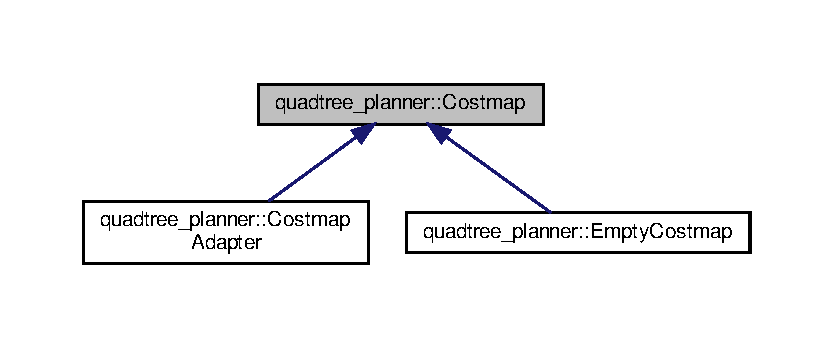
\includegraphics[width=350pt]{classquadtree__planner_1_1Costmap__inherit__graph}
\end{center}
\end{figure}
\subsection*{Public Member Functions}
\begin{DoxyCompactItemize}
\item 
virtual unsigned \hyperlink{classquadtree__planner_1_1Costmap_ada8d9915ad1b73637730fe65be8d291d}{get\+Cost} (unsigned int x, unsigned int y) const =0
\begin{DoxyCompactList}\small\item\em Get the cost of a cell in the costmap. \end{DoxyCompactList}\item 
virtual double \hyperlink{classquadtree__planner_1_1Costmap_a86720bf9d3de86f59af0229d706763c1}{get\+Size\+In\+MetersX} () const =0
\begin{DoxyCompactList}\small\item\em Get the size of the costmap in x direction in meters. \end{DoxyCompactList}\item 
virtual double \hyperlink{classquadtree__planner_1_1Costmap_ac0767c6851d243d8d12a8a0dbd2d022b}{get\+Size\+In\+MetersY} () const =0
\begin{DoxyCompactList}\small\item\em Get the size of the costmap in y direction in meters. \end{DoxyCompactList}\item 
virtual unsigned int \hyperlink{classquadtree__planner_1_1Costmap_aa78086776637e7472d5ca8ae44f5c2f0}{get\+Size\+In\+CellsX} () const =0
\begin{DoxyCompactList}\small\item\em Get the size of the costmap in x direction in cells. \end{DoxyCompactList}\item 
virtual unsigned int \hyperlink{classquadtree__planner_1_1Costmap_a5c07589004856b158dbbe38470562bfe}{get\+Size\+In\+CellsY} () const =0
\begin{DoxyCompactList}\small\item\em Get the size of the costmap in y direction in cells. \end{DoxyCompactList}\item 
virtual void \hyperlink{classquadtree__planner_1_1Costmap_a5384641291709625c2215144e97cf69c}{set\+Cost} (unsigned int mx, unsigned int my, unsigned char cost) const =0
\begin{DoxyCompactList}\small\item\em Set the cost of a cell in the costmap. \end{DoxyCompactList}\item 
virtual double \hyperlink{classquadtree__planner_1_1Costmap_aaef2845def8e7320a7fa576e9efab289}{get\+Resolution} () const =0
\begin{DoxyCompactList}\small\item\em Get resolution of the costmap, in meters per cell. \end{DoxyCompactList}\item 
virtual bool \hyperlink{classquadtree__planner_1_1Costmap_aba601c58933da74c707214d4dba2925a}{world\+To\+Map} (double wx, double wy, unsigned int \&mx, unsigned int \&my) const =0
\begin{DoxyCompactList}\small\item\em Convert from world coordinates to map coordinates. \end{DoxyCompactList}\item 
virtual void \hyperlink{classquadtree__planner_1_1Costmap_af82ccc7c15bd2cb9092e002ac6998eba}{map\+To\+World} (unsigned int mx, unsigned int my, double \&wx, double \&wy) const =0
\begin{DoxyCompactList}\small\item\em Convert from map coordinates to world coordinates. \end{DoxyCompactList}\item 
virtual bool \hyperlink{classquadtree__planner_1_1Costmap_ad6251247260f19389a1fa547c9b0d956}{save\+Map} (std\+::string file\+\_\+name) const =0
\begin{DoxyCompactList}\small\item\em the costmap to a file as a greyscale image \end{DoxyCompactList}\item 
virtual double \hyperlink{classquadtree__planner_1_1Costmap_a8fda39ff20cf58f6700705dae7bd3a0b}{get\+OriginX} () const =0
\begin{DoxyCompactList}\small\item\em the origin of the map in x direction in meters \end{DoxyCompactList}\item 
virtual double \hyperlink{classquadtree__planner_1_1Costmap_aa2b342e257504329321109b1822ca302}{get\+OriginY} () const =0
\begin{DoxyCompactList}\small\item\em the origin of the map in y direction in meters \end{DoxyCompactList}\end{DoxyCompactItemize}


\subsection{Detailed Description}
Associates costs with the points in the world. Largely corresponds to costmap\+\_\+2d/\+Costmap2D of the R\+OS navigation stack. 

\subsection{Member Function Documentation}
\mbox{\Hypertarget{classquadtree__planner_1_1Costmap_ada8d9915ad1b73637730fe65be8d291d}\label{classquadtree__planner_1_1Costmap_ada8d9915ad1b73637730fe65be8d291d}} 
\index{quadtree\+\_\+planner\+::\+Costmap@{quadtree\+\_\+planner\+::\+Costmap}!get\+Cost@{get\+Cost}}
\index{get\+Cost@{get\+Cost}!quadtree\+\_\+planner\+::\+Costmap@{quadtree\+\_\+planner\+::\+Costmap}}
\subsubsection{\texorpdfstring{get\+Cost()}{getCost()}}
{\footnotesize\ttfamily virtual unsigned quadtree\+\_\+planner\+::\+Costmap\+::get\+Cost (\begin{DoxyParamCaption}\item[{unsigned int}]{x,  }\item[{unsigned int}]{y }\end{DoxyParamCaption}) const\hspace{0.3cm}{\ttfamily [pure virtual]}}



Get the cost of a cell in the costmap. 


\begin{DoxyParams}{Parameters}
{\em mx} & The x coordinate of the cell \\
\hline
{\em my} & The y coordinate of the cell \\
\hline
\end{DoxyParams}
\begin{DoxyReturn}{Returns}
The cost of the cell 
\end{DoxyReturn}


Implemented in \hyperlink{classquadtree__planner_1_1CostmapAdapter_af5b15c508adabc428aabde14253c9468}{quadtree\+\_\+planner\+::\+Costmap\+Adapter}, and \hyperlink{classquadtree__planner_1_1EmptyCostmap_a2d952b1e51adc413b4ca767e4cd082dc}{quadtree\+\_\+planner\+::\+Empty\+Costmap}.

\mbox{\Hypertarget{classquadtree__planner_1_1Costmap_a8fda39ff20cf58f6700705dae7bd3a0b}\label{classquadtree__planner_1_1Costmap_a8fda39ff20cf58f6700705dae7bd3a0b}} 
\index{quadtree\+\_\+planner\+::\+Costmap@{quadtree\+\_\+planner\+::\+Costmap}!get\+OriginX@{get\+OriginX}}
\index{get\+OriginX@{get\+OriginX}!quadtree\+\_\+planner\+::\+Costmap@{quadtree\+\_\+planner\+::\+Costmap}}
\subsubsection{\texorpdfstring{get\+Origin\+X()}{getOriginX()}}
{\footnotesize\ttfamily virtual double quadtree\+\_\+planner\+::\+Costmap\+::get\+OriginX (\begin{DoxyParamCaption}{ }\end{DoxyParamCaption}) const\hspace{0.3cm}{\ttfamily [pure virtual]}}



the origin of the map in x direction in meters 

\begin{DoxyReturn}{Returns}
origin of the map in x direction in meters 
\end{DoxyReturn}


Implemented in \hyperlink{classquadtree__planner_1_1CostmapAdapter_ad63fb92c24234eb69b7672a7c9f15d26}{quadtree\+\_\+planner\+::\+Costmap\+Adapter}.

\mbox{\Hypertarget{classquadtree__planner_1_1Costmap_aa2b342e257504329321109b1822ca302}\label{classquadtree__planner_1_1Costmap_aa2b342e257504329321109b1822ca302}} 
\index{quadtree\+\_\+planner\+::\+Costmap@{quadtree\+\_\+planner\+::\+Costmap}!get\+OriginY@{get\+OriginY}}
\index{get\+OriginY@{get\+OriginY}!quadtree\+\_\+planner\+::\+Costmap@{quadtree\+\_\+planner\+::\+Costmap}}
\subsubsection{\texorpdfstring{get\+Origin\+Y()}{getOriginY()}}
{\footnotesize\ttfamily virtual double quadtree\+\_\+planner\+::\+Costmap\+::get\+OriginY (\begin{DoxyParamCaption}{ }\end{DoxyParamCaption}) const\hspace{0.3cm}{\ttfamily [pure virtual]}}



the origin of the map in y direction in meters 

\begin{DoxyReturn}{Returns}
origin of the map in y direction in meters 
\end{DoxyReturn}


Implemented in \hyperlink{classquadtree__planner_1_1CostmapAdapter_a004ee5ebfac631b47f6d3987e933cd38}{quadtree\+\_\+planner\+::\+Costmap\+Adapter}.

\mbox{\Hypertarget{classquadtree__planner_1_1Costmap_aaef2845def8e7320a7fa576e9efab289}\label{classquadtree__planner_1_1Costmap_aaef2845def8e7320a7fa576e9efab289}} 
\index{quadtree\+\_\+planner\+::\+Costmap@{quadtree\+\_\+planner\+::\+Costmap}!get\+Resolution@{get\+Resolution}}
\index{get\+Resolution@{get\+Resolution}!quadtree\+\_\+planner\+::\+Costmap@{quadtree\+\_\+planner\+::\+Costmap}}
\subsubsection{\texorpdfstring{get\+Resolution()}{getResolution()}}
{\footnotesize\ttfamily virtual double quadtree\+\_\+planner\+::\+Costmap\+::get\+Resolution (\begin{DoxyParamCaption}{ }\end{DoxyParamCaption}) const\hspace{0.3cm}{\ttfamily [pure virtual]}}



Get resolution of the costmap, in meters per cell. 

\begin{DoxyReturn}{Returns}
resolution of the costmap, in meters per cell 
\end{DoxyReturn}


Implemented in \hyperlink{classquadtree__planner_1_1CostmapAdapter_abfe3febc6445cbbd2aa7379c8635539b}{quadtree\+\_\+planner\+::\+Costmap\+Adapter}, and \hyperlink{classquadtree__planner_1_1EmptyCostmap_a2401c36e2f5c93fc9ae3dde9fc9ac930}{quadtree\+\_\+planner\+::\+Empty\+Costmap}.

\mbox{\Hypertarget{classquadtree__planner_1_1Costmap_aa78086776637e7472d5ca8ae44f5c2f0}\label{classquadtree__planner_1_1Costmap_aa78086776637e7472d5ca8ae44f5c2f0}} 
\index{quadtree\+\_\+planner\+::\+Costmap@{quadtree\+\_\+planner\+::\+Costmap}!get\+Size\+In\+CellsX@{get\+Size\+In\+CellsX}}
\index{get\+Size\+In\+CellsX@{get\+Size\+In\+CellsX}!quadtree\+\_\+planner\+::\+Costmap@{quadtree\+\_\+planner\+::\+Costmap}}
\subsubsection{\texorpdfstring{get\+Size\+In\+Cells\+X()}{getSizeInCellsX()}}
{\footnotesize\ttfamily virtual unsigned int quadtree\+\_\+planner\+::\+Costmap\+::get\+Size\+In\+CellsX (\begin{DoxyParamCaption}{ }\end{DoxyParamCaption}) const\hspace{0.3cm}{\ttfamily [pure virtual]}}



Get the size of the costmap in x direction in cells. 

\begin{DoxyReturn}{Returns}
size of the costmap in x direction in cells 
\end{DoxyReturn}


Implemented in \hyperlink{classquadtree__planner_1_1CostmapAdapter_a376b9bddbf47474be992170d06e008d7}{quadtree\+\_\+planner\+::\+Costmap\+Adapter}, and \hyperlink{classquadtree__planner_1_1EmptyCostmap_a41621ddd089ca5112d02c1315241534c}{quadtree\+\_\+planner\+::\+Empty\+Costmap}.

\mbox{\Hypertarget{classquadtree__planner_1_1Costmap_a5c07589004856b158dbbe38470562bfe}\label{classquadtree__planner_1_1Costmap_a5c07589004856b158dbbe38470562bfe}} 
\index{quadtree\+\_\+planner\+::\+Costmap@{quadtree\+\_\+planner\+::\+Costmap}!get\+Size\+In\+CellsY@{get\+Size\+In\+CellsY}}
\index{get\+Size\+In\+CellsY@{get\+Size\+In\+CellsY}!quadtree\+\_\+planner\+::\+Costmap@{quadtree\+\_\+planner\+::\+Costmap}}
\subsubsection{\texorpdfstring{get\+Size\+In\+Cells\+Y()}{getSizeInCellsY()}}
{\footnotesize\ttfamily virtual unsigned int quadtree\+\_\+planner\+::\+Costmap\+::get\+Size\+In\+CellsY (\begin{DoxyParamCaption}{ }\end{DoxyParamCaption}) const\hspace{0.3cm}{\ttfamily [pure virtual]}}



Get the size of the costmap in y direction in cells. 

\begin{DoxyReturn}{Returns}
size of the costmap in y direction in cells 
\end{DoxyReturn}


Implemented in \hyperlink{classquadtree__planner_1_1CostmapAdapter_a7d54b4b74b3057018408550c1116066e}{quadtree\+\_\+planner\+::\+Costmap\+Adapter}, and \hyperlink{classquadtree__planner_1_1EmptyCostmap_a2e3c5ddaaaee218d1cccf2a72dbe633f}{quadtree\+\_\+planner\+::\+Empty\+Costmap}.

\mbox{\Hypertarget{classquadtree__planner_1_1Costmap_a86720bf9d3de86f59af0229d706763c1}\label{classquadtree__planner_1_1Costmap_a86720bf9d3de86f59af0229d706763c1}} 
\index{quadtree\+\_\+planner\+::\+Costmap@{quadtree\+\_\+planner\+::\+Costmap}!get\+Size\+In\+MetersX@{get\+Size\+In\+MetersX}}
\index{get\+Size\+In\+MetersX@{get\+Size\+In\+MetersX}!quadtree\+\_\+planner\+::\+Costmap@{quadtree\+\_\+planner\+::\+Costmap}}
\subsubsection{\texorpdfstring{get\+Size\+In\+Meters\+X()}{getSizeInMetersX()}}
{\footnotesize\ttfamily virtual double quadtree\+\_\+planner\+::\+Costmap\+::get\+Size\+In\+MetersX (\begin{DoxyParamCaption}{ }\end{DoxyParamCaption}) const\hspace{0.3cm}{\ttfamily [pure virtual]}}



Get the size of the costmap in x direction in meters. 

\begin{DoxyReturn}{Returns}
size of the costmap in x direction in meters 
\end{DoxyReturn}


Implemented in \hyperlink{classquadtree__planner_1_1CostmapAdapter_a360c5f4047437c2fb69b91e598e0aecf}{quadtree\+\_\+planner\+::\+Costmap\+Adapter}, and \hyperlink{classquadtree__planner_1_1EmptyCostmap_ae7bbb00b36630b65f3e5d5d55a519fdd}{quadtree\+\_\+planner\+::\+Empty\+Costmap}.

\mbox{\Hypertarget{classquadtree__planner_1_1Costmap_ac0767c6851d243d8d12a8a0dbd2d022b}\label{classquadtree__planner_1_1Costmap_ac0767c6851d243d8d12a8a0dbd2d022b}} 
\index{quadtree\+\_\+planner\+::\+Costmap@{quadtree\+\_\+planner\+::\+Costmap}!get\+Size\+In\+MetersY@{get\+Size\+In\+MetersY}}
\index{get\+Size\+In\+MetersY@{get\+Size\+In\+MetersY}!quadtree\+\_\+planner\+::\+Costmap@{quadtree\+\_\+planner\+::\+Costmap}}
\subsubsection{\texorpdfstring{get\+Size\+In\+Meters\+Y()}{getSizeInMetersY()}}
{\footnotesize\ttfamily virtual double quadtree\+\_\+planner\+::\+Costmap\+::get\+Size\+In\+MetersY (\begin{DoxyParamCaption}{ }\end{DoxyParamCaption}) const\hspace{0.3cm}{\ttfamily [pure virtual]}}



Get the size of the costmap in y direction in meters. 

\begin{DoxyReturn}{Returns}
size of the costmap in y direction in meters 
\end{DoxyReturn}


Implemented in \hyperlink{classquadtree__planner_1_1CostmapAdapter_aa253651d1b4596009ca26009e7ad28f8}{quadtree\+\_\+planner\+::\+Costmap\+Adapter}, and \hyperlink{classquadtree__planner_1_1EmptyCostmap_aec6c2b1a739b6475f21219d688bc0b54}{quadtree\+\_\+planner\+::\+Empty\+Costmap}.

\mbox{\Hypertarget{classquadtree__planner_1_1Costmap_af82ccc7c15bd2cb9092e002ac6998eba}\label{classquadtree__planner_1_1Costmap_af82ccc7c15bd2cb9092e002ac6998eba}} 
\index{quadtree\+\_\+planner\+::\+Costmap@{quadtree\+\_\+planner\+::\+Costmap}!map\+To\+World@{map\+To\+World}}
\index{map\+To\+World@{map\+To\+World}!quadtree\+\_\+planner\+::\+Costmap@{quadtree\+\_\+planner\+::\+Costmap}}
\subsubsection{\texorpdfstring{map\+To\+World()}{mapToWorld()}}
{\footnotesize\ttfamily virtual void quadtree\+\_\+planner\+::\+Costmap\+::map\+To\+World (\begin{DoxyParamCaption}\item[{unsigned int}]{mx,  }\item[{unsigned int}]{my,  }\item[{double \&}]{wx,  }\item[{double \&}]{wy }\end{DoxyParamCaption}) const\hspace{0.3cm}{\ttfamily [pure virtual]}}



Convert from map coordinates to world coordinates. 


\begin{DoxyParams}{Parameters}
{\em mx} & The x map coordinate \\
\hline
{\em my} & The y map coordinate \\
\hline
{\em wx} & Will be set to the associated world x coordinate \\
\hline
{\em wy} & Will be set to the associated world y coordinate \\
\hline
\end{DoxyParams}


Implemented in \hyperlink{classquadtree__planner_1_1CostmapAdapter_aa3b530c60bd8565e32166642e5e37663}{quadtree\+\_\+planner\+::\+Costmap\+Adapter}.

\mbox{\Hypertarget{classquadtree__planner_1_1Costmap_ad6251247260f19389a1fa547c9b0d956}\label{classquadtree__planner_1_1Costmap_ad6251247260f19389a1fa547c9b0d956}} 
\index{quadtree\+\_\+planner\+::\+Costmap@{quadtree\+\_\+planner\+::\+Costmap}!save\+Map@{save\+Map}}
\index{save\+Map@{save\+Map}!quadtree\+\_\+planner\+::\+Costmap@{quadtree\+\_\+planner\+::\+Costmap}}
\subsubsection{\texorpdfstring{save\+Map()}{saveMap()}}
{\footnotesize\ttfamily virtual bool quadtree\+\_\+planner\+::\+Costmap\+::save\+Map (\begin{DoxyParamCaption}\item[{std\+::string}]{file\+\_\+name }\end{DoxyParamCaption}) const\hspace{0.3cm}{\ttfamily [pure virtual]}}



the costmap to a file as a greyscale image 


\begin{DoxyParams}{Parameters}
{\em file\+\_\+name} & path to file where the image shall be stored (e.\+g. as .pgm) \\
\hline
\end{DoxyParams}
\begin{DoxyReturn}{Returns}

\end{DoxyReturn}


Implemented in \hyperlink{classquadtree__planner_1_1CostmapAdapter_a11201eaf5094483113acf5d195923893}{quadtree\+\_\+planner\+::\+Costmap\+Adapter}.

\mbox{\Hypertarget{classquadtree__planner_1_1Costmap_a5384641291709625c2215144e97cf69c}\label{classquadtree__planner_1_1Costmap_a5384641291709625c2215144e97cf69c}} 
\index{quadtree\+\_\+planner\+::\+Costmap@{quadtree\+\_\+planner\+::\+Costmap}!set\+Cost@{set\+Cost}}
\index{set\+Cost@{set\+Cost}!quadtree\+\_\+planner\+::\+Costmap@{quadtree\+\_\+planner\+::\+Costmap}}
\subsubsection{\texorpdfstring{set\+Cost()}{setCost()}}
{\footnotesize\ttfamily virtual void quadtree\+\_\+planner\+::\+Costmap\+::set\+Cost (\begin{DoxyParamCaption}\item[{unsigned int}]{mx,  }\item[{unsigned int}]{my,  }\item[{unsigned char}]{cost }\end{DoxyParamCaption}) const\hspace{0.3cm}{\ttfamily [pure virtual]}}



Set the cost of a cell in the costmap. 


\begin{DoxyParams}{Parameters}
{\em mx} & The x coordinate of the cell \\
\hline
{\em my} & The y coordinate of the cell \\
\hline
\end{DoxyParams}


Implemented in \hyperlink{classquadtree__planner_1_1CostmapAdapter_a816f4036c5a67297c72302ad4329b98b}{quadtree\+\_\+planner\+::\+Costmap\+Adapter}.

\mbox{\Hypertarget{classquadtree__planner_1_1Costmap_aba601c58933da74c707214d4dba2925a}\label{classquadtree__planner_1_1Costmap_aba601c58933da74c707214d4dba2925a}} 
\index{quadtree\+\_\+planner\+::\+Costmap@{quadtree\+\_\+planner\+::\+Costmap}!world\+To\+Map@{world\+To\+Map}}
\index{world\+To\+Map@{world\+To\+Map}!quadtree\+\_\+planner\+::\+Costmap@{quadtree\+\_\+planner\+::\+Costmap}}
\subsubsection{\texorpdfstring{world\+To\+Map()}{worldToMap()}}
{\footnotesize\ttfamily virtual bool quadtree\+\_\+planner\+::\+Costmap\+::world\+To\+Map (\begin{DoxyParamCaption}\item[{double}]{wx,  }\item[{double}]{wy,  }\item[{unsigned int \&}]{mx,  }\item[{unsigned int \&}]{my }\end{DoxyParamCaption}) const\hspace{0.3cm}{\ttfamily [pure virtual]}}



Convert from world coordinates to map coordinates. 


\begin{DoxyParams}{Parameters}
{\em wx} & The x world coordinate \\
\hline
{\em wy} & The y world coordinate \\
\hline
{\em mx} & Will be set to the associated map x coordinate \\
\hline
{\em my} & Will be set to the associated map y coordinate \\
\hline
\end{DoxyParams}
\begin{DoxyReturn}{Returns}
True if the conversion was successful (legal bounds) false otherwise 
\end{DoxyReturn}


Implemented in \hyperlink{classquadtree__planner_1_1CostmapAdapter_a422624b4df8d3fa267eb367389b73751}{quadtree\+\_\+planner\+::\+Costmap\+Adapter}, and \hyperlink{classquadtree__planner_1_1EmptyCostmap_a329690825d4e3789189dc0b99c891786}{quadtree\+\_\+planner\+::\+Empty\+Costmap}.



The documentation for this class was generated from the following file\+:\begin{DoxyCompactItemize}
\item 
/home/maximilian/\+Roboy\+Repo\+Devel\+Planning/src/quadtree\+\_\+planner/include/quadtree\+\_\+planner/costmap.\+h\end{DoxyCompactItemize}

\hypertarget{classquadtree__planner_1_1CostmapAdapter}{}\section{quadtree\+\_\+planner\+:\+:Costmap\+Adapter Class Reference}
\label{classquadtree__planner_1_1CostmapAdapter}\index{quadtree\+\_\+planner\+::\+Costmap\+Adapter@{quadtree\+\_\+planner\+::\+Costmap\+Adapter}}


{\ttfamily \#include $<$costmap.\+h$>$}



Inheritance diagram for quadtree\+\_\+planner\+:\+:Costmap\+Adapter\+:\nopagebreak
\begin{figure}[H]
\begin{center}
\leavevmode
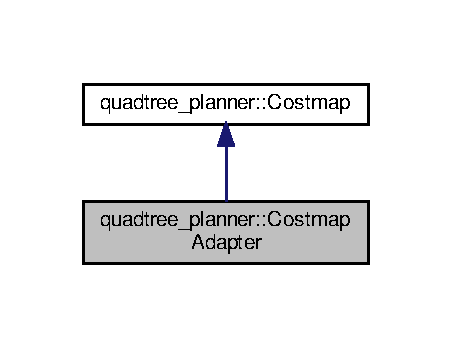
\includegraphics[width=217pt]{classquadtree__planner_1_1CostmapAdapter__inherit__graph}
\end{center}
\end{figure}


Collaboration diagram for quadtree\+\_\+planner\+:\+:Costmap\+Adapter\+:\nopagebreak
\begin{figure}[H]
\begin{center}
\leavevmode
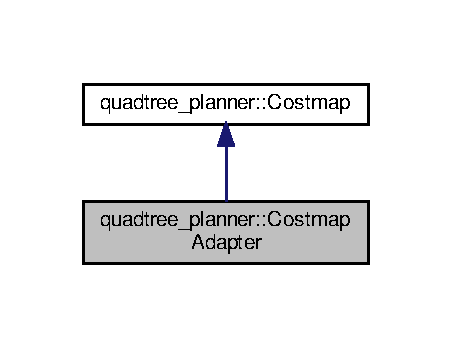
\includegraphics[width=217pt]{classquadtree__planner_1_1CostmapAdapter__coll__graph}
\end{center}
\end{figure}
\subsection*{Public Member Functions}
\begin{DoxyCompactItemize}
\item 
\hyperlink{classquadtree__planner_1_1CostmapAdapter_a3efe5b09f0fc3c5f3c0df1557854a8d7}{Costmap\+Adapter} (costmap\+\_\+2d\+::\+Costmap2D $\ast$costmap)
\begin{DoxyCompactList}\small\item\em Constructor for \hyperlink{classquadtree__planner_1_1CostmapAdapter}{Costmap\+Adapter} class. \end{DoxyCompactList}\item 
unsigned int \hyperlink{classquadtree__planner_1_1CostmapAdapter_af5b15c508adabc428aabde14253c9468}{get\+Cost} (unsigned int x, unsigned int y) const override
\begin{DoxyCompactList}\small\item\em Get the cost of a cell in the costmap. \end{DoxyCompactList}\item 
double \hyperlink{classquadtree__planner_1_1CostmapAdapter_a360c5f4047437c2fb69b91e598e0aecf}{get\+Size\+In\+MetersX} () const override
\begin{DoxyCompactList}\small\item\em Get the size of the costmap in x direction in meters. \end{DoxyCompactList}\item 
double \hyperlink{classquadtree__planner_1_1CostmapAdapter_aa253651d1b4596009ca26009e7ad28f8}{get\+Size\+In\+MetersY} () const override
\begin{DoxyCompactList}\small\item\em Get the size of the costmap in y direction in meters. \end{DoxyCompactList}\item 
unsigned int \hyperlink{classquadtree__planner_1_1CostmapAdapter_a376b9bddbf47474be992170d06e008d7}{get\+Size\+In\+CellsX} () const override
\begin{DoxyCompactList}\small\item\em Get the size of the costmap in x direction in cells. \end{DoxyCompactList}\item 
unsigned int \hyperlink{classquadtree__planner_1_1CostmapAdapter_a7d54b4b74b3057018408550c1116066e}{get\+Size\+In\+CellsY} () const override
\begin{DoxyCompactList}\small\item\em Get the size of the costmap in y direction in cells. \end{DoxyCompactList}\item 
double \hyperlink{classquadtree__planner_1_1CostmapAdapter_abfe3febc6445cbbd2aa7379c8635539b}{get\+Resolution} () const override
\begin{DoxyCompactList}\small\item\em Get resolution of the costmap, in meters per cell. \end{DoxyCompactList}\item 
void \hyperlink{classquadtree__planner_1_1CostmapAdapter_a816f4036c5a67297c72302ad4329b98b}{set\+Cost} (unsigned int mx, unsigned int my, unsigned char cost) const override
\begin{DoxyCompactList}\small\item\em Set the cost of a cell in the costmap. \end{DoxyCompactList}\item 
bool \hyperlink{classquadtree__planner_1_1CostmapAdapter_a422624b4df8d3fa267eb367389b73751}{world\+To\+Map} (double wx, double wy, unsigned int \&mx, unsigned int \&my) const override
\begin{DoxyCompactList}\small\item\em Convert from world coordinates to map coordinates. \end{DoxyCompactList}\item 
void \hyperlink{classquadtree__planner_1_1CostmapAdapter_aa3b530c60bd8565e32166642e5e37663}{map\+To\+World} (unsigned int mx, unsigned int my, double \&wx, double \&wy) const override
\begin{DoxyCompactList}\small\item\em Convert from map coordinates to world coordinates. \end{DoxyCompactList}\item 
bool \hyperlink{classquadtree__planner_1_1CostmapAdapter_a11201eaf5094483113acf5d195923893}{save\+Map} (std\+::string file\+\_\+name) const override
\begin{DoxyCompactList}\small\item\em the costmap to a file as a greyscale image \end{DoxyCompactList}\item 
double \hyperlink{classquadtree__planner_1_1CostmapAdapter_ad63fb92c24234eb69b7672a7c9f15d26}{get\+OriginX} () const override
\begin{DoxyCompactList}\small\item\em the origin of the map in x direction in meters \end{DoxyCompactList}\item 
double \hyperlink{classquadtree__planner_1_1CostmapAdapter_a004ee5ebfac631b47f6d3987e933cd38}{get\+OriginY} () const override
\begin{DoxyCompactList}\small\item\em the origin of the map in y direction in meters \end{DoxyCompactList}\end{DoxyCompactItemize}


\subsection{Detailed Description}
An adapter that fullfils the \hyperlink{classquadtree__planner_1_1Costmap}{Costmap} interfaces and delegates to a costmap\+\_\+2d/\+Costmap2D impolemenation. 

\subsection{Constructor \& Destructor Documentation}
\mbox{\Hypertarget{classquadtree__planner_1_1CostmapAdapter_a3efe5b09f0fc3c5f3c0df1557854a8d7}\label{classquadtree__planner_1_1CostmapAdapter_a3efe5b09f0fc3c5f3c0df1557854a8d7}} 
\index{quadtree\+\_\+planner\+::\+Costmap\+Adapter@{quadtree\+\_\+planner\+::\+Costmap\+Adapter}!Costmap\+Adapter@{Costmap\+Adapter}}
\index{Costmap\+Adapter@{Costmap\+Adapter}!quadtree\+\_\+planner\+::\+Costmap\+Adapter@{quadtree\+\_\+planner\+::\+Costmap\+Adapter}}
\subsubsection{\texorpdfstring{Costmap\+Adapter()}{CostmapAdapter()}}
{\footnotesize\ttfamily quadtree\+\_\+planner\+::\+Costmap\+Adapter\+::\+Costmap\+Adapter (\begin{DoxyParamCaption}\item[{costmap\+\_\+2d\+::\+Costmap2D $\ast$}]{costmap }\end{DoxyParamCaption})}



Constructor for \hyperlink{classquadtree__planner_1_1CostmapAdapter}{Costmap\+Adapter} class. 


\begin{DoxyParams}{Parameters}
{\em costmap} & pointer to costmap\+\_\+2d ros object instance \\
\hline
\end{DoxyParams}


\subsection{Member Function Documentation}
\mbox{\Hypertarget{classquadtree__planner_1_1CostmapAdapter_af5b15c508adabc428aabde14253c9468}\label{classquadtree__planner_1_1CostmapAdapter_af5b15c508adabc428aabde14253c9468}} 
\index{quadtree\+\_\+planner\+::\+Costmap\+Adapter@{quadtree\+\_\+planner\+::\+Costmap\+Adapter}!get\+Cost@{get\+Cost}}
\index{get\+Cost@{get\+Cost}!quadtree\+\_\+planner\+::\+Costmap\+Adapter@{quadtree\+\_\+planner\+::\+Costmap\+Adapter}}
\subsubsection{\texorpdfstring{get\+Cost()}{getCost()}}
{\footnotesize\ttfamily unsigned int quadtree\+\_\+planner\+::\+Costmap\+Adapter\+::get\+Cost (\begin{DoxyParamCaption}\item[{unsigned int}]{x,  }\item[{unsigned int}]{y }\end{DoxyParamCaption}) const\hspace{0.3cm}{\ttfamily [override]}, {\ttfamily [virtual]}}



Get the cost of a cell in the costmap. 


\begin{DoxyParams}{Parameters}
{\em mx} & The x coordinate of the cell \\
\hline
{\em my} & The y coordinate of the cell \\
\hline
\end{DoxyParams}
\begin{DoxyReturn}{Returns}
The cost of the cell 
\end{DoxyReturn}


Implements \hyperlink{classquadtree__planner_1_1Costmap_ada8d9915ad1b73637730fe65be8d291d}{quadtree\+\_\+planner\+::\+Costmap}.

\mbox{\Hypertarget{classquadtree__planner_1_1CostmapAdapter_ad63fb92c24234eb69b7672a7c9f15d26}\label{classquadtree__planner_1_1CostmapAdapter_ad63fb92c24234eb69b7672a7c9f15d26}} 
\index{quadtree\+\_\+planner\+::\+Costmap\+Adapter@{quadtree\+\_\+planner\+::\+Costmap\+Adapter}!get\+OriginX@{get\+OriginX}}
\index{get\+OriginX@{get\+OriginX}!quadtree\+\_\+planner\+::\+Costmap\+Adapter@{quadtree\+\_\+planner\+::\+Costmap\+Adapter}}
\subsubsection{\texorpdfstring{get\+Origin\+X()}{getOriginX()}}
{\footnotesize\ttfamily double quadtree\+\_\+planner\+::\+Costmap\+Adapter\+::get\+OriginX (\begin{DoxyParamCaption}{ }\end{DoxyParamCaption}) const\hspace{0.3cm}{\ttfamily [override]}, {\ttfamily [virtual]}}



the origin of the map in x direction in meters 

\begin{DoxyReturn}{Returns}
origin of the map in x direction in meters 
\end{DoxyReturn}


Implements \hyperlink{classquadtree__planner_1_1Costmap_a8fda39ff20cf58f6700705dae7bd3a0b}{quadtree\+\_\+planner\+::\+Costmap}.

\mbox{\Hypertarget{classquadtree__planner_1_1CostmapAdapter_a004ee5ebfac631b47f6d3987e933cd38}\label{classquadtree__planner_1_1CostmapAdapter_a004ee5ebfac631b47f6d3987e933cd38}} 
\index{quadtree\+\_\+planner\+::\+Costmap\+Adapter@{quadtree\+\_\+planner\+::\+Costmap\+Adapter}!get\+OriginY@{get\+OriginY}}
\index{get\+OriginY@{get\+OriginY}!quadtree\+\_\+planner\+::\+Costmap\+Adapter@{quadtree\+\_\+planner\+::\+Costmap\+Adapter}}
\subsubsection{\texorpdfstring{get\+Origin\+Y()}{getOriginY()}}
{\footnotesize\ttfamily double quadtree\+\_\+planner\+::\+Costmap\+Adapter\+::get\+OriginY (\begin{DoxyParamCaption}{ }\end{DoxyParamCaption}) const\hspace{0.3cm}{\ttfamily [override]}, {\ttfamily [virtual]}}



the origin of the map in y direction in meters 

\begin{DoxyReturn}{Returns}
origin of the map in y direction in meters 
\end{DoxyReturn}


Implements \hyperlink{classquadtree__planner_1_1Costmap_aa2b342e257504329321109b1822ca302}{quadtree\+\_\+planner\+::\+Costmap}.

\mbox{\Hypertarget{classquadtree__planner_1_1CostmapAdapter_abfe3febc6445cbbd2aa7379c8635539b}\label{classquadtree__planner_1_1CostmapAdapter_abfe3febc6445cbbd2aa7379c8635539b}} 
\index{quadtree\+\_\+planner\+::\+Costmap\+Adapter@{quadtree\+\_\+planner\+::\+Costmap\+Adapter}!get\+Resolution@{get\+Resolution}}
\index{get\+Resolution@{get\+Resolution}!quadtree\+\_\+planner\+::\+Costmap\+Adapter@{quadtree\+\_\+planner\+::\+Costmap\+Adapter}}
\subsubsection{\texorpdfstring{get\+Resolution()}{getResolution()}}
{\footnotesize\ttfamily double quadtree\+\_\+planner\+::\+Costmap\+Adapter\+::get\+Resolution (\begin{DoxyParamCaption}{ }\end{DoxyParamCaption}) const\hspace{0.3cm}{\ttfamily [override]}, {\ttfamily [virtual]}}



Get resolution of the costmap, in meters per cell. 

\begin{DoxyReturn}{Returns}
resolution of the costmap, in meters per cell 
\end{DoxyReturn}


Implements \hyperlink{classquadtree__planner_1_1Costmap_aaef2845def8e7320a7fa576e9efab289}{quadtree\+\_\+planner\+::\+Costmap}.

\mbox{\Hypertarget{classquadtree__planner_1_1CostmapAdapter_a376b9bddbf47474be992170d06e008d7}\label{classquadtree__planner_1_1CostmapAdapter_a376b9bddbf47474be992170d06e008d7}} 
\index{quadtree\+\_\+planner\+::\+Costmap\+Adapter@{quadtree\+\_\+planner\+::\+Costmap\+Adapter}!get\+Size\+In\+CellsX@{get\+Size\+In\+CellsX}}
\index{get\+Size\+In\+CellsX@{get\+Size\+In\+CellsX}!quadtree\+\_\+planner\+::\+Costmap\+Adapter@{quadtree\+\_\+planner\+::\+Costmap\+Adapter}}
\subsubsection{\texorpdfstring{get\+Size\+In\+Cells\+X()}{getSizeInCellsX()}}
{\footnotesize\ttfamily uint quadtree\+\_\+planner\+::\+Costmap\+Adapter\+::get\+Size\+In\+CellsX (\begin{DoxyParamCaption}{ }\end{DoxyParamCaption}) const\hspace{0.3cm}{\ttfamily [override]}, {\ttfamily [virtual]}}



Get the size of the costmap in x direction in cells. 

\begin{DoxyReturn}{Returns}
size of the costmap in x direction in cells 
\end{DoxyReturn}


Implements \hyperlink{classquadtree__planner_1_1Costmap_aa78086776637e7472d5ca8ae44f5c2f0}{quadtree\+\_\+planner\+::\+Costmap}.

\mbox{\Hypertarget{classquadtree__planner_1_1CostmapAdapter_a7d54b4b74b3057018408550c1116066e}\label{classquadtree__planner_1_1CostmapAdapter_a7d54b4b74b3057018408550c1116066e}} 
\index{quadtree\+\_\+planner\+::\+Costmap\+Adapter@{quadtree\+\_\+planner\+::\+Costmap\+Adapter}!get\+Size\+In\+CellsY@{get\+Size\+In\+CellsY}}
\index{get\+Size\+In\+CellsY@{get\+Size\+In\+CellsY}!quadtree\+\_\+planner\+::\+Costmap\+Adapter@{quadtree\+\_\+planner\+::\+Costmap\+Adapter}}
\subsubsection{\texorpdfstring{get\+Size\+In\+Cells\+Y()}{getSizeInCellsY()}}
{\footnotesize\ttfamily uint quadtree\+\_\+planner\+::\+Costmap\+Adapter\+::get\+Size\+In\+CellsY (\begin{DoxyParamCaption}{ }\end{DoxyParamCaption}) const\hspace{0.3cm}{\ttfamily [override]}, {\ttfamily [virtual]}}



Get the size of the costmap in y direction in cells. 

\begin{DoxyReturn}{Returns}
size of the costmap in y direction in cells 
\end{DoxyReturn}


Implements \hyperlink{classquadtree__planner_1_1Costmap_a5c07589004856b158dbbe38470562bfe}{quadtree\+\_\+planner\+::\+Costmap}.

\mbox{\Hypertarget{classquadtree__planner_1_1CostmapAdapter_a360c5f4047437c2fb69b91e598e0aecf}\label{classquadtree__planner_1_1CostmapAdapter_a360c5f4047437c2fb69b91e598e0aecf}} 
\index{quadtree\+\_\+planner\+::\+Costmap\+Adapter@{quadtree\+\_\+planner\+::\+Costmap\+Adapter}!get\+Size\+In\+MetersX@{get\+Size\+In\+MetersX}}
\index{get\+Size\+In\+MetersX@{get\+Size\+In\+MetersX}!quadtree\+\_\+planner\+::\+Costmap\+Adapter@{quadtree\+\_\+planner\+::\+Costmap\+Adapter}}
\subsubsection{\texorpdfstring{get\+Size\+In\+Meters\+X()}{getSizeInMetersX()}}
{\footnotesize\ttfamily double quadtree\+\_\+planner\+::\+Costmap\+Adapter\+::get\+Size\+In\+MetersX (\begin{DoxyParamCaption}{ }\end{DoxyParamCaption}) const\hspace{0.3cm}{\ttfamily [override]}, {\ttfamily [virtual]}}



Get the size of the costmap in x direction in meters. 

\begin{DoxyReturn}{Returns}
size of the costmap in x direction in meters 
\end{DoxyReturn}


Implements \hyperlink{classquadtree__planner_1_1Costmap_a86720bf9d3de86f59af0229d706763c1}{quadtree\+\_\+planner\+::\+Costmap}.

\mbox{\Hypertarget{classquadtree__planner_1_1CostmapAdapter_aa253651d1b4596009ca26009e7ad28f8}\label{classquadtree__planner_1_1CostmapAdapter_aa253651d1b4596009ca26009e7ad28f8}} 
\index{quadtree\+\_\+planner\+::\+Costmap\+Adapter@{quadtree\+\_\+planner\+::\+Costmap\+Adapter}!get\+Size\+In\+MetersY@{get\+Size\+In\+MetersY}}
\index{get\+Size\+In\+MetersY@{get\+Size\+In\+MetersY}!quadtree\+\_\+planner\+::\+Costmap\+Adapter@{quadtree\+\_\+planner\+::\+Costmap\+Adapter}}
\subsubsection{\texorpdfstring{get\+Size\+In\+Meters\+Y()}{getSizeInMetersY()}}
{\footnotesize\ttfamily double quadtree\+\_\+planner\+::\+Costmap\+Adapter\+::get\+Size\+In\+MetersY (\begin{DoxyParamCaption}{ }\end{DoxyParamCaption}) const\hspace{0.3cm}{\ttfamily [override]}, {\ttfamily [virtual]}}



Get the size of the costmap in y direction in meters. 

\begin{DoxyReturn}{Returns}
size of the costmap in y direction in meters 
\end{DoxyReturn}


Implements \hyperlink{classquadtree__planner_1_1Costmap_ac0767c6851d243d8d12a8a0dbd2d022b}{quadtree\+\_\+planner\+::\+Costmap}.

\mbox{\Hypertarget{classquadtree__planner_1_1CostmapAdapter_aa3b530c60bd8565e32166642e5e37663}\label{classquadtree__planner_1_1CostmapAdapter_aa3b530c60bd8565e32166642e5e37663}} 
\index{quadtree\+\_\+planner\+::\+Costmap\+Adapter@{quadtree\+\_\+planner\+::\+Costmap\+Adapter}!map\+To\+World@{map\+To\+World}}
\index{map\+To\+World@{map\+To\+World}!quadtree\+\_\+planner\+::\+Costmap\+Adapter@{quadtree\+\_\+planner\+::\+Costmap\+Adapter}}
\subsubsection{\texorpdfstring{map\+To\+World()}{mapToWorld()}}
{\footnotesize\ttfamily void quadtree\+\_\+planner\+::\+Costmap\+Adapter\+::map\+To\+World (\begin{DoxyParamCaption}\item[{unsigned int}]{mx,  }\item[{unsigned int}]{my,  }\item[{double \&}]{wx,  }\item[{double \&}]{wy }\end{DoxyParamCaption}) const\hspace{0.3cm}{\ttfamily [override]}, {\ttfamily [virtual]}}



Convert from map coordinates to world coordinates. 


\begin{DoxyParams}{Parameters}
{\em mx} & The x map coordinate \\
\hline
{\em my} & The y map coordinate \\
\hline
{\em wx} & Will be set to the associated world x coordinate \\
\hline
{\em wy} & Will be set to the associated world y coordinate \\
\hline
\end{DoxyParams}


Implements \hyperlink{classquadtree__planner_1_1Costmap_af82ccc7c15bd2cb9092e002ac6998eba}{quadtree\+\_\+planner\+::\+Costmap}.

\mbox{\Hypertarget{classquadtree__planner_1_1CostmapAdapter_a11201eaf5094483113acf5d195923893}\label{classquadtree__planner_1_1CostmapAdapter_a11201eaf5094483113acf5d195923893}} 
\index{quadtree\+\_\+planner\+::\+Costmap\+Adapter@{quadtree\+\_\+planner\+::\+Costmap\+Adapter}!save\+Map@{save\+Map}}
\index{save\+Map@{save\+Map}!quadtree\+\_\+planner\+::\+Costmap\+Adapter@{quadtree\+\_\+planner\+::\+Costmap\+Adapter}}
\subsubsection{\texorpdfstring{save\+Map()}{saveMap()}}
{\footnotesize\ttfamily bool quadtree\+\_\+planner\+::\+Costmap\+Adapter\+::save\+Map (\begin{DoxyParamCaption}\item[{std\+::string}]{file\+\_\+name }\end{DoxyParamCaption}) const\hspace{0.3cm}{\ttfamily [override]}, {\ttfamily [virtual]}}



the costmap to a file as a greyscale image 


\begin{DoxyParams}{Parameters}
{\em file\+\_\+name} & path to file where the image shall be stored (e.\+g. as .pgm) \\
\hline
\end{DoxyParams}
\begin{DoxyReturn}{Returns}

\end{DoxyReturn}


Implements \hyperlink{classquadtree__planner_1_1Costmap_ad6251247260f19389a1fa547c9b0d956}{quadtree\+\_\+planner\+::\+Costmap}.

\mbox{\Hypertarget{classquadtree__planner_1_1CostmapAdapter_a816f4036c5a67297c72302ad4329b98b}\label{classquadtree__planner_1_1CostmapAdapter_a816f4036c5a67297c72302ad4329b98b}} 
\index{quadtree\+\_\+planner\+::\+Costmap\+Adapter@{quadtree\+\_\+planner\+::\+Costmap\+Adapter}!set\+Cost@{set\+Cost}}
\index{set\+Cost@{set\+Cost}!quadtree\+\_\+planner\+::\+Costmap\+Adapter@{quadtree\+\_\+planner\+::\+Costmap\+Adapter}}
\subsubsection{\texorpdfstring{set\+Cost()}{setCost()}}
{\footnotesize\ttfamily void quadtree\+\_\+planner\+::\+Costmap\+Adapter\+::set\+Cost (\begin{DoxyParamCaption}\item[{unsigned int}]{mx,  }\item[{unsigned int}]{my,  }\item[{unsigned char}]{cost }\end{DoxyParamCaption}) const\hspace{0.3cm}{\ttfamily [override]}, {\ttfamily [virtual]}}



Set the cost of a cell in the costmap. 


\begin{DoxyParams}{Parameters}
{\em mx} & The x coordinate of the cell \\
\hline
{\em my} & The y coordinate of the cell \\
\hline
\end{DoxyParams}


Implements \hyperlink{classquadtree__planner_1_1Costmap_a5384641291709625c2215144e97cf69c}{quadtree\+\_\+planner\+::\+Costmap}.

\mbox{\Hypertarget{classquadtree__planner_1_1CostmapAdapter_a422624b4df8d3fa267eb367389b73751}\label{classquadtree__planner_1_1CostmapAdapter_a422624b4df8d3fa267eb367389b73751}} 
\index{quadtree\+\_\+planner\+::\+Costmap\+Adapter@{quadtree\+\_\+planner\+::\+Costmap\+Adapter}!world\+To\+Map@{world\+To\+Map}}
\index{world\+To\+Map@{world\+To\+Map}!quadtree\+\_\+planner\+::\+Costmap\+Adapter@{quadtree\+\_\+planner\+::\+Costmap\+Adapter}}
\subsubsection{\texorpdfstring{world\+To\+Map()}{worldToMap()}}
{\footnotesize\ttfamily bool quadtree\+\_\+planner\+::\+Costmap\+Adapter\+::world\+To\+Map (\begin{DoxyParamCaption}\item[{double}]{wx,  }\item[{double}]{wy,  }\item[{unsigned int \&}]{mx,  }\item[{unsigned int \&}]{my }\end{DoxyParamCaption}) const\hspace{0.3cm}{\ttfamily [override]}, {\ttfamily [virtual]}}



Convert from world coordinates to map coordinates. 


\begin{DoxyParams}{Parameters}
{\em wx} & The x world coordinate \\
\hline
{\em wy} & The y world coordinate \\
\hline
{\em mx} & Will be set to the associated map x coordinate \\
\hline
{\em my} & Will be set to the associated map y coordinate \\
\hline
\end{DoxyParams}
\begin{DoxyReturn}{Returns}
True if the conversion was successful (legal bounds) false otherwise 
\end{DoxyReturn}


Implements \hyperlink{classquadtree__planner_1_1Costmap_aba601c58933da74c707214d4dba2925a}{quadtree\+\_\+planner\+::\+Costmap}.



The documentation for this class was generated from the following files\+:\begin{DoxyCompactItemize}
\item 
/home/maximilian/\+Roboy\+Repo\+Devel\+Planning/src/quadtree\+\_\+planner/include/quadtree\+\_\+planner/costmap.\+h\item 
/home/maximilian/\+Roboy\+Repo\+Devel\+Planning/src/quadtree\+\_\+planner/src/costmap.\+cpp\end{DoxyCompactItemize}

\hypertarget{structDubinsIntermediateResults}{}\section{Dubins\+Intermediate\+Results Struct Reference}
\label{structDubinsIntermediateResults}\index{Dubins\+Intermediate\+Results@{Dubins\+Intermediate\+Results}}
\subsection*{Public Attributes}
\begin{DoxyCompactItemize}
\item 
\mbox{\Hypertarget{structDubinsIntermediateResults_a16dd90fd03de98085a5a2fe20462bdb7}\label{structDubinsIntermediateResults_a16dd90fd03de98085a5a2fe20462bdb7}} 
double {\bfseries alpha}
\item 
\mbox{\Hypertarget{structDubinsIntermediateResults_a3cdf7760c671e13f89d39a9a7797bb27}\label{structDubinsIntermediateResults_a3cdf7760c671e13f89d39a9a7797bb27}} 
double {\bfseries beta}
\item 
\mbox{\Hypertarget{structDubinsIntermediateResults_a2c7907bf15d843630ab3ac72c008dc29}\label{structDubinsIntermediateResults_a2c7907bf15d843630ab3ac72c008dc29}} 
double {\bfseries d}
\item 
\mbox{\Hypertarget{structDubinsIntermediateResults_a8f48ddc917c92cdc085e8307bb614c3c}\label{structDubinsIntermediateResults_a8f48ddc917c92cdc085e8307bb614c3c}} 
double {\bfseries sa}
\item 
\mbox{\Hypertarget{structDubinsIntermediateResults_afaa830d0fac94e976b9c73617ef81c23}\label{structDubinsIntermediateResults_afaa830d0fac94e976b9c73617ef81c23}} 
double {\bfseries sb}
\item 
\mbox{\Hypertarget{structDubinsIntermediateResults_ad90b052827792e3593993570f1af378f}\label{structDubinsIntermediateResults_ad90b052827792e3593993570f1af378f}} 
double {\bfseries ca}
\item 
\mbox{\Hypertarget{structDubinsIntermediateResults_aa0b40e6890ad6ca9bb6b8393f1cdba29}\label{structDubinsIntermediateResults_aa0b40e6890ad6ca9bb6b8393f1cdba29}} 
double {\bfseries cb}
\item 
\mbox{\Hypertarget{structDubinsIntermediateResults_abbfbd766bb26dd03b571bce328032f92}\label{structDubinsIntermediateResults_abbfbd766bb26dd03b571bce328032f92}} 
double {\bfseries c\+\_\+ab}
\item 
\mbox{\Hypertarget{structDubinsIntermediateResults_aee0ab71f744ccb8551d3d409c2c38391}\label{structDubinsIntermediateResults_aee0ab71f744ccb8551d3d409c2c38391}} 
double {\bfseries d\+\_\+sq}
\end{DoxyCompactItemize}


The documentation for this struct was generated from the following file\+:\begin{DoxyCompactItemize}
\item 
/home/maximilian/\+Roboy\+Repo\+Devel\+Planning/src/quadtree\+\_\+planner/src/dubins.\+c\end{DoxyCompactItemize}

\hypertarget{structDubinsPath}{}\section{Dubins\+Path Struct Reference}
\label{structDubinsPath}\index{Dubins\+Path@{Dubins\+Path}}
\subsection*{Public Attributes}
\begin{DoxyCompactItemize}
\item 
\mbox{\Hypertarget{structDubinsPath_aabcbfbb58406794577c58b00f6109263}\label{structDubinsPath_aabcbfbb58406794577c58b00f6109263}} 
double {\bfseries qi} \mbox{[}3\mbox{]}
\item 
\mbox{\Hypertarget{structDubinsPath_a0e88cf654931b652566e497a156e0c91}\label{structDubinsPath_a0e88cf654931b652566e497a156e0c91}} 
double {\bfseries param} \mbox{[}3\mbox{]}
\item 
\mbox{\Hypertarget{structDubinsPath_a7731666554b2a029e60717f26a8defb8}\label{structDubinsPath_a7731666554b2a029e60717f26a8defb8}} 
double {\bfseries rho}
\item 
\mbox{\Hypertarget{structDubinsPath_af1de248d28f35c6784a8f9a3c99db25b}\label{structDubinsPath_af1de248d28f35c6784a8f9a3c99db25b}} 
Dubins\+Path\+Type {\bfseries type}
\end{DoxyCompactItemize}


The documentation for this struct was generated from the following file\+:\begin{DoxyCompactItemize}
\item 
/home/maximilian/\+Roboy\+Repo\+Devel\+Planning/src/quadtree\+\_\+planner/include/quadtree\+\_\+planner/dubins.\+h\end{DoxyCompactItemize}

\hypertarget{structquadtree__planner_1_1DubinsSubpath}{}\section{quadtree\+\_\+planner\+:\+:Dubins\+Subpath Struct Reference}
\label{structquadtree__planner_1_1DubinsSubpath}\index{quadtree\+\_\+planner\+::\+Dubins\+Subpath@{quadtree\+\_\+planner\+::\+Dubins\+Subpath}}


{\ttfamily \#include $<$utils.\+h$>$}



Collaboration diagram for quadtree\+\_\+planner\+:\+:Dubins\+Subpath\+:\nopagebreak
\begin{figure}[H]
\begin{center}
\leavevmode
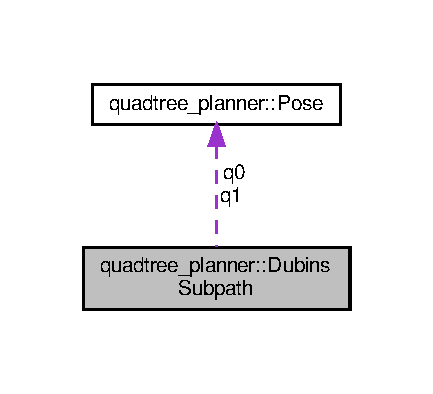
\includegraphics[width=208pt]{structquadtree__planner_1_1DubinsSubpath__coll__graph}
\end{center}
\end{figure}
\subsection*{Public Member Functions}
\begin{DoxyCompactItemize}
\item 
\mbox{\Hypertarget{structquadtree__planner_1_1DubinsSubpath_aca184e2e5a7ddc1d699941154e4b76bb}\label{structquadtree__planner_1_1DubinsSubpath_aca184e2e5a7ddc1d699941154e4b76bb}} 
{\bfseries Dubins\+Subpath} (\hyperlink{structquadtree__planner_1_1Pose}{Pose} q0, \hyperlink{structquadtree__planner_1_1Pose}{Pose} q1, double turning\+\_\+radius, Dubins\+Path\+Type dubins\+Path\+Type)
\end{DoxyCompactItemize}
\subsection*{Public Attributes}
\begin{DoxyCompactItemize}
\item 
\mbox{\Hypertarget{structquadtree__planner_1_1DubinsSubpath_a855b4da40a33f3f00972d27cffd46676}\label{structquadtree__planner_1_1DubinsSubpath_a855b4da40a33f3f00972d27cffd46676}} 
\hyperlink{structquadtree__planner_1_1Pose}{Pose} {\bfseries q0}
\item 
\mbox{\Hypertarget{structquadtree__planner_1_1DubinsSubpath_a21654f1004522b7dbacca9459ccf3b23}\label{structquadtree__planner_1_1DubinsSubpath_a21654f1004522b7dbacca9459ccf3b23}} 
\hyperlink{structquadtree__planner_1_1Pose}{Pose} {\bfseries q1}
\item 
\mbox{\Hypertarget{structquadtree__planner_1_1DubinsSubpath_a1287c19670d9d00eedfb8a8086a06754}\label{structquadtree__planner_1_1DubinsSubpath_a1287c19670d9d00eedfb8a8086a06754}} 
double {\bfseries turning\+\_\+radius}
\item 
\mbox{\Hypertarget{structquadtree__planner_1_1DubinsSubpath_ae7ea561e580756e838676b3c4f39566c}\label{structquadtree__planner_1_1DubinsSubpath_ae7ea561e580756e838676b3c4f39566c}} 
Dubins\+Path\+Type {\bfseries dubins\+Path\+Type}
\end{DoxyCompactItemize}


\subsection{Detailed Description}
Container for storing \hyperlink{structquadtree__planner_1_1DubinsSubpath}{Dubins\+Subpath} consisting of start and goal pose, turning radius and Dubins\+Path\+Type 

The documentation for this struct was generated from the following files\+:\begin{DoxyCompactItemize}
\item 
/home/maximilian/\+Roboy\+Repo\+Devel\+Planning/src/quadtree\+\_\+planner/include/quadtree\+\_\+planner/utils.\+h\item 
/home/maximilian/\+Roboy\+Repo\+Devel\+Planning/src/quadtree\+\_\+planner/src/utils.\+cpp\end{DoxyCompactItemize}

\hypertarget{classquadtree__planner_1_1EmptyCostmap}{}\section{quadtree\+\_\+planner\+:\+:Empty\+Costmap Class Reference}
\label{classquadtree__planner_1_1EmptyCostmap}\index{quadtree\+\_\+planner\+::\+Empty\+Costmap@{quadtree\+\_\+planner\+::\+Empty\+Costmap}}


{\ttfamily \#include $<$costmap.\+h$>$}



Inheritance diagram for quadtree\+\_\+planner\+:\+:Empty\+Costmap\+:\nopagebreak
\begin{figure}[H]
\begin{center}
\leavevmode
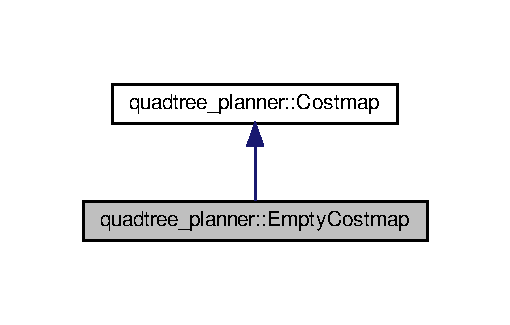
\includegraphics[width=245pt]{classquadtree__planner_1_1EmptyCostmap__inherit__graph}
\end{center}
\end{figure}


Collaboration diagram for quadtree\+\_\+planner\+:\+:Empty\+Costmap\+:\nopagebreak
\begin{figure}[H]
\begin{center}
\leavevmode
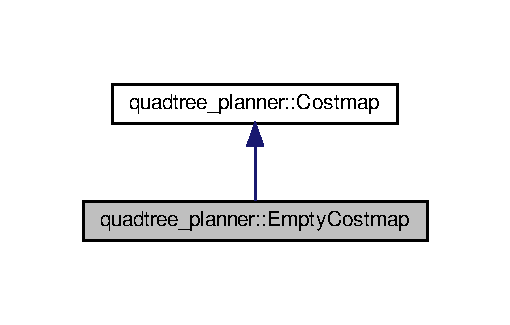
\includegraphics[width=245pt]{classquadtree__planner_1_1EmptyCostmap__coll__graph}
\end{center}
\end{figure}
\subsection*{Public Member Functions}
\begin{DoxyCompactItemize}
\item 
\hyperlink{classquadtree__planner_1_1EmptyCostmap_ac76dfd72c0366cc6ea8cf63a9adde273}{Empty\+Costmap} (unsigned int sizeX, unsigned int sizeY, double resolution)
\begin{DoxyCompactList}\small\item\em Constructor for \hyperlink{classquadtree__planner_1_1EmptyCostmap}{Empty\+Costmap} class. \end{DoxyCompactList}\item 
unsigned int \hyperlink{classquadtree__planner_1_1EmptyCostmap_a2d952b1e51adc413b4ca767e4cd082dc}{get\+Cost} (unsigned int x, unsigned int y) const override
\begin{DoxyCompactList}\small\item\em Get the cost of a cell in the costmap. \end{DoxyCompactList}\item 
double \hyperlink{classquadtree__planner_1_1EmptyCostmap_ae7bbb00b36630b65f3e5d5d55a519fdd}{get\+Size\+In\+MetersX} () const override
\begin{DoxyCompactList}\small\item\em Get the size of the costmap in x direction in meters. \end{DoxyCompactList}\item 
double \hyperlink{classquadtree__planner_1_1EmptyCostmap_aec6c2b1a739b6475f21219d688bc0b54}{get\+Size\+In\+MetersY} () const override
\begin{DoxyCompactList}\small\item\em Get the size of the costmap in y direction in meters. \end{DoxyCompactList}\item 
unsigned int \hyperlink{classquadtree__planner_1_1EmptyCostmap_a41621ddd089ca5112d02c1315241534c}{get\+Size\+In\+CellsX} () const override
\begin{DoxyCompactList}\small\item\em Get the size of the costmap in x direction in cells. \end{DoxyCompactList}\item 
unsigned int \hyperlink{classquadtree__planner_1_1EmptyCostmap_a2e3c5ddaaaee218d1cccf2a72dbe633f}{get\+Size\+In\+CellsY} () const override
\begin{DoxyCompactList}\small\item\em Get the size of the costmap in y direction in cells. \end{DoxyCompactList}\item 
double \hyperlink{classquadtree__planner_1_1EmptyCostmap_a2401c36e2f5c93fc9ae3dde9fc9ac930}{get\+Resolution} () const override
\begin{DoxyCompactList}\small\item\em Get resolution of the costmap, in meters per cell. \end{DoxyCompactList}\item 
bool \hyperlink{classquadtree__planner_1_1EmptyCostmap_a329690825d4e3789189dc0b99c891786}{world\+To\+Map} (double wx, double wy, unsigned int \&mx, unsigned int \&my) const override
\begin{DoxyCompactList}\small\item\em Convert from world coordinates to map coordinates. \end{DoxyCompactList}\end{DoxyCompactItemize}


\subsection{Detailed Description}
A stub costmap used for testing purposes. 

\subsection{Constructor \& Destructor Documentation}
\mbox{\Hypertarget{classquadtree__planner_1_1EmptyCostmap_ac76dfd72c0366cc6ea8cf63a9adde273}\label{classquadtree__planner_1_1EmptyCostmap_ac76dfd72c0366cc6ea8cf63a9adde273}} 
\index{quadtree\+\_\+planner\+::\+Empty\+Costmap@{quadtree\+\_\+planner\+::\+Empty\+Costmap}!Empty\+Costmap@{Empty\+Costmap}}
\index{Empty\+Costmap@{Empty\+Costmap}!quadtree\+\_\+planner\+::\+Empty\+Costmap@{quadtree\+\_\+planner\+::\+Empty\+Costmap}}
\subsubsection{\texorpdfstring{Empty\+Costmap()}{EmptyCostmap()}}
{\footnotesize\ttfamily quadtree\+\_\+planner\+::\+Empty\+Costmap\+::\+Empty\+Costmap (\begin{DoxyParamCaption}\item[{unsigned int}]{sizeX,  }\item[{unsigned int}]{sizeY,  }\item[{double}]{resolution }\end{DoxyParamCaption})}



Constructor for \hyperlink{classquadtree__planner_1_1EmptyCostmap}{Empty\+Costmap} class. 


\begin{DoxyParams}{Parameters}
{\em sizeX} & size of the costmap in cells in x direction \\
\hline
{\em sizeY} & size of the costmap in cells in y direction \\
\hline
{\em resolution} & resolution of the costmap, in meters per cell \\
\hline
\end{DoxyParams}


\subsection{Member Function Documentation}
\mbox{\Hypertarget{classquadtree__planner_1_1EmptyCostmap_a2d952b1e51adc413b4ca767e4cd082dc}\label{classquadtree__planner_1_1EmptyCostmap_a2d952b1e51adc413b4ca767e4cd082dc}} 
\index{quadtree\+\_\+planner\+::\+Empty\+Costmap@{quadtree\+\_\+planner\+::\+Empty\+Costmap}!get\+Cost@{get\+Cost}}
\index{get\+Cost@{get\+Cost}!quadtree\+\_\+planner\+::\+Empty\+Costmap@{quadtree\+\_\+planner\+::\+Empty\+Costmap}}
\subsubsection{\texorpdfstring{get\+Cost()}{getCost()}}
{\footnotesize\ttfamily unsigned int quadtree\+\_\+planner\+::\+Empty\+Costmap\+::get\+Cost (\begin{DoxyParamCaption}\item[{unsigned int}]{x,  }\item[{unsigned int}]{y }\end{DoxyParamCaption}) const\hspace{0.3cm}{\ttfamily [override]}, {\ttfamily [virtual]}}



Get the cost of a cell in the costmap. 


\begin{DoxyParams}{Parameters}
{\em mx} & The x coordinate of the cell \\
\hline
{\em my} & The y coordinate of the cell \\
\hline
\end{DoxyParams}
\begin{DoxyReturn}{Returns}
The cost of the cell 
\end{DoxyReturn}


Implements \hyperlink{classquadtree__planner_1_1Costmap_ada8d9915ad1b73637730fe65be8d291d}{quadtree\+\_\+planner\+::\+Costmap}.

\mbox{\Hypertarget{classquadtree__planner_1_1EmptyCostmap_a2401c36e2f5c93fc9ae3dde9fc9ac930}\label{classquadtree__planner_1_1EmptyCostmap_a2401c36e2f5c93fc9ae3dde9fc9ac930}} 
\index{quadtree\+\_\+planner\+::\+Empty\+Costmap@{quadtree\+\_\+planner\+::\+Empty\+Costmap}!get\+Resolution@{get\+Resolution}}
\index{get\+Resolution@{get\+Resolution}!quadtree\+\_\+planner\+::\+Empty\+Costmap@{quadtree\+\_\+planner\+::\+Empty\+Costmap}}
\subsubsection{\texorpdfstring{get\+Resolution()}{getResolution()}}
{\footnotesize\ttfamily double quadtree\+\_\+planner\+::\+Empty\+Costmap\+::get\+Resolution (\begin{DoxyParamCaption}{ }\end{DoxyParamCaption}) const\hspace{0.3cm}{\ttfamily [override]}, {\ttfamily [virtual]}}



Get resolution of the costmap, in meters per cell. 

\begin{DoxyReturn}{Returns}
resolution of the costmap, in meters per cell 
\end{DoxyReturn}


Implements \hyperlink{classquadtree__planner_1_1Costmap_aaef2845def8e7320a7fa576e9efab289}{quadtree\+\_\+planner\+::\+Costmap}.

\mbox{\Hypertarget{classquadtree__planner_1_1EmptyCostmap_a41621ddd089ca5112d02c1315241534c}\label{classquadtree__planner_1_1EmptyCostmap_a41621ddd089ca5112d02c1315241534c}} 
\index{quadtree\+\_\+planner\+::\+Empty\+Costmap@{quadtree\+\_\+planner\+::\+Empty\+Costmap}!get\+Size\+In\+CellsX@{get\+Size\+In\+CellsX}}
\index{get\+Size\+In\+CellsX@{get\+Size\+In\+CellsX}!quadtree\+\_\+planner\+::\+Empty\+Costmap@{quadtree\+\_\+planner\+::\+Empty\+Costmap}}
\subsubsection{\texorpdfstring{get\+Size\+In\+Cells\+X()}{getSizeInCellsX()}}
{\footnotesize\ttfamily unsigned int quadtree\+\_\+planner\+::\+Empty\+Costmap\+::get\+Size\+In\+CellsX (\begin{DoxyParamCaption}{ }\end{DoxyParamCaption}) const\hspace{0.3cm}{\ttfamily [override]}, {\ttfamily [virtual]}}



Get the size of the costmap in x direction in cells. 

\begin{DoxyReturn}{Returns}
size of the costmap in x direction in cells 
\end{DoxyReturn}


Implements \hyperlink{classquadtree__planner_1_1Costmap_aa78086776637e7472d5ca8ae44f5c2f0}{quadtree\+\_\+planner\+::\+Costmap}.

\mbox{\Hypertarget{classquadtree__planner_1_1EmptyCostmap_a2e3c5ddaaaee218d1cccf2a72dbe633f}\label{classquadtree__planner_1_1EmptyCostmap_a2e3c5ddaaaee218d1cccf2a72dbe633f}} 
\index{quadtree\+\_\+planner\+::\+Empty\+Costmap@{quadtree\+\_\+planner\+::\+Empty\+Costmap}!get\+Size\+In\+CellsY@{get\+Size\+In\+CellsY}}
\index{get\+Size\+In\+CellsY@{get\+Size\+In\+CellsY}!quadtree\+\_\+planner\+::\+Empty\+Costmap@{quadtree\+\_\+planner\+::\+Empty\+Costmap}}
\subsubsection{\texorpdfstring{get\+Size\+In\+Cells\+Y()}{getSizeInCellsY()}}
{\footnotesize\ttfamily unsigned int quadtree\+\_\+planner\+::\+Empty\+Costmap\+::get\+Size\+In\+CellsY (\begin{DoxyParamCaption}{ }\end{DoxyParamCaption}) const\hspace{0.3cm}{\ttfamily [override]}, {\ttfamily [virtual]}}



Get the size of the costmap in y direction in cells. 

\begin{DoxyReturn}{Returns}
size of the costmap in y direction in cells 
\end{DoxyReturn}


Implements \hyperlink{classquadtree__planner_1_1Costmap_a5c07589004856b158dbbe38470562bfe}{quadtree\+\_\+planner\+::\+Costmap}.

\mbox{\Hypertarget{classquadtree__planner_1_1EmptyCostmap_ae7bbb00b36630b65f3e5d5d55a519fdd}\label{classquadtree__planner_1_1EmptyCostmap_ae7bbb00b36630b65f3e5d5d55a519fdd}} 
\index{quadtree\+\_\+planner\+::\+Empty\+Costmap@{quadtree\+\_\+planner\+::\+Empty\+Costmap}!get\+Size\+In\+MetersX@{get\+Size\+In\+MetersX}}
\index{get\+Size\+In\+MetersX@{get\+Size\+In\+MetersX}!quadtree\+\_\+planner\+::\+Empty\+Costmap@{quadtree\+\_\+planner\+::\+Empty\+Costmap}}
\subsubsection{\texorpdfstring{get\+Size\+In\+Meters\+X()}{getSizeInMetersX()}}
{\footnotesize\ttfamily double quadtree\+\_\+planner\+::\+Empty\+Costmap\+::get\+Size\+In\+MetersX (\begin{DoxyParamCaption}{ }\end{DoxyParamCaption}) const\hspace{0.3cm}{\ttfamily [override]}, {\ttfamily [virtual]}}



Get the size of the costmap in x direction in meters. 

\begin{DoxyReturn}{Returns}
size of the costmap in x direction in meters 
\end{DoxyReturn}


Implements \hyperlink{classquadtree__planner_1_1Costmap_a86720bf9d3de86f59af0229d706763c1}{quadtree\+\_\+planner\+::\+Costmap}.

\mbox{\Hypertarget{classquadtree__planner_1_1EmptyCostmap_aec6c2b1a739b6475f21219d688bc0b54}\label{classquadtree__planner_1_1EmptyCostmap_aec6c2b1a739b6475f21219d688bc0b54}} 
\index{quadtree\+\_\+planner\+::\+Empty\+Costmap@{quadtree\+\_\+planner\+::\+Empty\+Costmap}!get\+Size\+In\+MetersY@{get\+Size\+In\+MetersY}}
\index{get\+Size\+In\+MetersY@{get\+Size\+In\+MetersY}!quadtree\+\_\+planner\+::\+Empty\+Costmap@{quadtree\+\_\+planner\+::\+Empty\+Costmap}}
\subsubsection{\texorpdfstring{get\+Size\+In\+Meters\+Y()}{getSizeInMetersY()}}
{\footnotesize\ttfamily double quadtree\+\_\+planner\+::\+Empty\+Costmap\+::get\+Size\+In\+MetersY (\begin{DoxyParamCaption}{ }\end{DoxyParamCaption}) const\hspace{0.3cm}{\ttfamily [override]}, {\ttfamily [virtual]}}



Get the size of the costmap in y direction in meters. 

\begin{DoxyReturn}{Returns}
size of the costmap in y direction in meters 
\end{DoxyReturn}


Implements \hyperlink{classquadtree__planner_1_1Costmap_ac0767c6851d243d8d12a8a0dbd2d022b}{quadtree\+\_\+planner\+::\+Costmap}.

\mbox{\Hypertarget{classquadtree__planner_1_1EmptyCostmap_a329690825d4e3789189dc0b99c891786}\label{classquadtree__planner_1_1EmptyCostmap_a329690825d4e3789189dc0b99c891786}} 
\index{quadtree\+\_\+planner\+::\+Empty\+Costmap@{quadtree\+\_\+planner\+::\+Empty\+Costmap}!world\+To\+Map@{world\+To\+Map}}
\index{world\+To\+Map@{world\+To\+Map}!quadtree\+\_\+planner\+::\+Empty\+Costmap@{quadtree\+\_\+planner\+::\+Empty\+Costmap}}
\subsubsection{\texorpdfstring{world\+To\+Map()}{worldToMap()}}
{\footnotesize\ttfamily bool quadtree\+\_\+planner\+::\+Empty\+Costmap\+::world\+To\+Map (\begin{DoxyParamCaption}\item[{double}]{wx,  }\item[{double}]{wy,  }\item[{unsigned int \&}]{mx,  }\item[{unsigned int \&}]{my }\end{DoxyParamCaption}) const\hspace{0.3cm}{\ttfamily [override]}, {\ttfamily [virtual]}}



Convert from world coordinates to map coordinates. 


\begin{DoxyParams}{Parameters}
{\em wx} & The x world coordinate \\
\hline
{\em wy} & The y world coordinate \\
\hline
{\em mx} & Will be set to the associated map x coordinate \\
\hline
{\em my} & Will be set to the associated map y coordinate \\
\hline
\end{DoxyParams}
\begin{DoxyReturn}{Returns}
True if the conversion was successful (legal bounds) false otherwise 
\end{DoxyReturn}


Implements \hyperlink{classquadtree__planner_1_1Costmap_aba601c58933da74c707214d4dba2925a}{quadtree\+\_\+planner\+::\+Costmap}.



The documentation for this class was generated from the following files\+:\begin{DoxyCompactItemize}
\item 
/home/maximilian/\+Roboy\+Repo\+Devel\+Planning/src/quadtree\+\_\+planner/include/quadtree\+\_\+planner/costmap.\+h\item 
/home/maximilian/\+Roboy\+Repo\+Devel\+Planning/src/quadtree\+\_\+planner/src/costmap.\+cpp\end{DoxyCompactItemize}

\hypertarget{structstd_1_1hash_3_01quadtree__planner_1_1Pose_01_4}{}\section{std\+:\+:hash$<$ quadtree\+\_\+planner\+:\+:Pose $>$ Struct Template Reference}
\label{structstd_1_1hash_3_01quadtree__planner_1_1Pose_01_4}\index{std\+::hash$<$ quadtree\+\_\+planner\+::\+Pose $>$@{std\+::hash$<$ quadtree\+\_\+planner\+::\+Pose $>$}}
\subsection*{Public Member Functions}
\begin{DoxyCompactItemize}
\item 
\mbox{\Hypertarget{structstd_1_1hash_3_01quadtree__planner_1_1Pose_01_4_ac8874e34eca4fed9febfd628fb97b495}\label{structstd_1_1hash_3_01quadtree__planner_1_1Pose_01_4_ac8874e34eca4fed9febfd628fb97b495}} 
std\+::size\+\_\+t {\bfseries operator()} (const \hyperlink{structquadtree__planner_1_1Pose}{quadtree\+\_\+planner\+::\+Pose} \&pose) const
\end{DoxyCompactItemize}


The documentation for this struct was generated from the following file\+:\begin{DoxyCompactItemize}
\item 
/home/maximilian/\+Roboy\+Repo\+Devel\+Planning/src/quadtree\+\_\+planner/include/quadtree\+\_\+planner/utils.\+h\end{DoxyCompactItemize}

\hypertarget{structstd_1_1hash_3_01Quadtree__SearchCell_01_4}{}\section{std\+:\+:hash$<$ Quadtree\+\_\+\+Search\+Cell $>$ Struct Template Reference}
\label{structstd_1_1hash_3_01Quadtree__SearchCell_01_4}\index{std\+::hash$<$ Quadtree\+\_\+\+Search\+Cell $>$@{std\+::hash$<$ Quadtree\+\_\+\+Search\+Cell $>$}}
\subsection*{Public Member Functions}
\begin{DoxyCompactItemize}
\item 
\mbox{\Hypertarget{structstd_1_1hash_3_01Quadtree__SearchCell_01_4_a49f5ed24c48f19ae41ad1c70590525c7}\label{structstd_1_1hash_3_01Quadtree__SearchCell_01_4_a49f5ed24c48f19ae41ad1c70590525c7}} 
std\+::size\+\_\+t {\bfseries operator()} (const \hyperlink{classQuadtree__SearchCell}{Quadtree\+\_\+\+Search\+Cell} \&quad) const
\end{DoxyCompactItemize}


The documentation for this struct was generated from the following file\+:\begin{DoxyCompactItemize}
\item 
/home/maximilian/\+Roboy\+Repo\+Devel\+Planning/src/quadtree\+\_\+planner/include/quadtree\+\_\+planner/utils.\+h\end{DoxyCompactItemize}

\hypertarget{structquadtree__planner_1_1IntermediatePathAngles}{}\section{quadtree\+\_\+planner\+:\+:Intermediate\+Path\+Angles Struct Reference}
\label{structquadtree__planner_1_1IntermediatePathAngles}\index{quadtree\+\_\+planner\+::\+Intermediate\+Path\+Angles@{quadtree\+\_\+planner\+::\+Intermediate\+Path\+Angles}}


{\ttfamily \#include $<$utils.\+h$>$}

\subsection*{Public Member Functions}
\begin{DoxyCompactItemize}
\item 
\mbox{\Hypertarget{structquadtree__planner_1_1IntermediatePathAngles_a711619186b7354288876dc6b125b373d}\label{structquadtree__planner_1_1IntermediatePathAngles_a711619186b7354288876dc6b125b373d}} 
{\bfseries Intermediate\+Path\+Angles} (double first\+\_\+theta, double second\+\_\+theta, double path\+Length, Dubins\+Path\+Type dubins\+Path\+Type)
\item 
\mbox{\Hypertarget{structquadtree__planner_1_1IntermediatePathAngles_a20a2e352f73511256a9673875fdb746c}\label{structquadtree__planner_1_1IntermediatePathAngles_a20a2e352f73511256a9673875fdb746c}} 
bool {\bfseries operator==} (const \hyperlink{structquadtree__planner_1_1IntermediatePathAngles}{Intermediate\+Path\+Angles} \&other) const
\end{DoxyCompactItemize}
\subsection*{Public Attributes}
\begin{DoxyCompactItemize}
\item 
\mbox{\Hypertarget{structquadtree__planner_1_1IntermediatePathAngles_aa5247463531a95ae950bbf2a324f136a}\label{structquadtree__planner_1_1IntermediatePathAngles_aa5247463531a95ae950bbf2a324f136a}} 
double {\bfseries first\+\_\+theta}
\item 
\mbox{\Hypertarget{structquadtree__planner_1_1IntermediatePathAngles_a6325ee2585820d2122d755c9ae001d76}\label{structquadtree__planner_1_1IntermediatePathAngles_a6325ee2585820d2122d755c9ae001d76}} 
double {\bfseries second\+\_\+theta}
\item 
\mbox{\Hypertarget{structquadtree__planner_1_1IntermediatePathAngles_aef18855c07d94b77586c202a924a8c29}\label{structquadtree__planner_1_1IntermediatePathAngles_aef18855c07d94b77586c202a924a8c29}} 
double {\bfseries path\+Length}
\item 
\mbox{\Hypertarget{structquadtree__planner_1_1IntermediatePathAngles_aacc7c846a274efb649a5e03c811f3505}\label{structquadtree__planner_1_1IntermediatePathAngles_aacc7c846a274efb649a5e03c811f3505}} 
Dubins\+Path\+Type {\bfseries dubins\+Path\+Type}
\end{DoxyCompactItemize}
\subsection*{Friends}
\begin{DoxyCompactItemize}
\item 
\mbox{\Hypertarget{structquadtree__planner_1_1IntermediatePathAngles_aebdbac34a0623bf6750fdaf798c9122b}\label{structquadtree__planner_1_1IntermediatePathAngles_aebdbac34a0623bf6750fdaf798c9122b}} 
std\+::ostream \& {\bfseries operator$<$$<$} (std\+::ostream \&out, const \hyperlink{structquadtree__planner_1_1IntermediatePathAngles}{Intermediate\+Path\+Angles} \&intermediate\+Path\+Angles)
\end{DoxyCompactItemize}


\subsection{Detailed Description}
Container for storing valid angle combinations 

The documentation for this struct was generated from the following files\+:\begin{DoxyCompactItemize}
\item 
/home/maximilian/\+Roboy\+Repo\+Devel\+Planning/src/quadtree\+\_\+planner/include/quadtree\+\_\+planner/utils.\+h\item 
/home/maximilian/\+Roboy\+Repo\+Devel\+Planning/src/quadtree\+\_\+planner/src/utils.\+cpp\end{DoxyCompactItemize}

\hypertarget{structquadtree__planner_1_1IntermediatePaths}{}\section{quadtree\+\_\+planner\+:\+:Intermediate\+Paths Struct Reference}
\label{structquadtree__planner_1_1IntermediatePaths}\index{quadtree\+\_\+planner\+::\+Intermediate\+Paths@{quadtree\+\_\+planner\+::\+Intermediate\+Paths}}


{\ttfamily \#include $<$utils.\+h$>$}

\subsection*{Public Member Functions}
\begin{DoxyCompactItemize}
\item 
\mbox{\Hypertarget{structquadtree__planner_1_1IntermediatePaths_a5345b071f834cf2ca9fb0be256f39ea2}\label{structquadtree__planner_1_1IntermediatePaths_a5345b071f834cf2ca9fb0be256f39ea2}} 
{\bfseries Intermediate\+Paths} (int first\+\_\+index, int second\+\_\+index, std\+::vector$<$ \hyperlink{structquadtree__planner_1_1IntermediatePathAngles}{Intermediate\+Path\+Angles} $>$ intermediate\+Path\+Angles)
\item 
\mbox{\Hypertarget{structquadtree__planner_1_1IntermediatePaths_a6ed4e6644af54586e70e22d34aa9ddfb}\label{structquadtree__planner_1_1IntermediatePaths_a6ed4e6644af54586e70e22d34aa9ddfb}} 
bool {\bfseries operator==} (const \hyperlink{structquadtree__planner_1_1IntermediatePaths}{Intermediate\+Paths} \&other) const
\end{DoxyCompactItemize}
\subsection*{Public Attributes}
\begin{DoxyCompactItemize}
\item 
\mbox{\Hypertarget{structquadtree__planner_1_1IntermediatePaths_a5655dcf69ce97f40f99481f1a2cc8586}\label{structquadtree__planner_1_1IntermediatePaths_a5655dcf69ce97f40f99481f1a2cc8586}} 
int {\bfseries first\+\_\+index}
\item 
\mbox{\Hypertarget{structquadtree__planner_1_1IntermediatePaths_a6fc49ad9c13a2f3116c7cb288ff6405e}\label{structquadtree__planner_1_1IntermediatePaths_a6fc49ad9c13a2f3116c7cb288ff6405e}} 
int {\bfseries second\+\_\+index}
\item 
\mbox{\Hypertarget{structquadtree__planner_1_1IntermediatePaths_adf013ca83453d9254eb015814ca605a7}\label{structquadtree__planner_1_1IntermediatePaths_adf013ca83453d9254eb015814ca605a7}} 
std\+::vector$<$ \hyperlink{structquadtree__planner_1_1IntermediatePathAngles}{Intermediate\+Path\+Angles} $>$ {\bfseries intermediate\+Path\+Angles}
\end{DoxyCompactItemize}
\subsection*{Friends}
\begin{DoxyCompactItemize}
\item 
\mbox{\Hypertarget{structquadtree__planner_1_1IntermediatePaths_aad252649919945cbcff2c68113b7f442}\label{structquadtree__planner_1_1IntermediatePaths_aad252649919945cbcff2c68113b7f442}} 
std\+::ostream \& {\bfseries operator$<$$<$} (std\+::ostream \&out, const \hyperlink{structquadtree__planner_1_1IntermediatePaths}{Intermediate\+Paths} \&intermediate\+Paths)
\end{DoxyCompactItemize}


\subsection{Detailed Description}
Container for storing intermediate paths (possible angle combinations for each index combination) 

The documentation for this struct was generated from the following files\+:\begin{DoxyCompactItemize}
\item 
/home/maximilian/\+Roboy\+Repo\+Devel\+Planning/src/quadtree\+\_\+planner/include/quadtree\+\_\+planner/utils.\+h\item 
/home/maximilian/\+Roboy\+Repo\+Devel\+Planning/src/quadtree\+\_\+planner/src/utils.\+cpp\end{DoxyCompactItemize}

\hypertarget{structPoint}{}\section{Point Struct Reference}
\label{structPoint}\index{Point@{Point}}


{\ttfamily \#include $<$quadtree\+\_\+datastructure.\+h$>$}

\subsection*{Public Member Functions}
\begin{DoxyCompactItemize}
\item 
\mbox{\Hypertarget{structPoint_a5e6f571a8e78582930ceda907f4117cd}\label{structPoint_a5e6f571a8e78582930ceda907f4117cd}} 
{\bfseries Point} (unsigned int \+\_\+x, unsigned int \+\_\+y)
\item 
\mbox{\Hypertarget{structPoint_a3618cc973762afde2e8df59bff4a86ca}\label{structPoint_a3618cc973762afde2e8df59bff4a86ca}} 
bool {\bfseries operator==} (const \hyperlink{structPoint}{Point} \&p) const
\end{DoxyCompactItemize}
\subsection*{Public Attributes}
\begin{DoxyCompactItemize}
\item 
\mbox{\Hypertarget{structPoint_a81bb3d87085a9672879cfe4e58f7bff3}\label{structPoint_a81bb3d87085a9672879cfe4e58f7bff3}} 
unsigned int {\bfseries x}
\item 
\mbox{\Hypertarget{structPoint_aafc3278398083cef91e29bf68c7d6c87}\label{structPoint_aafc3278398083cef91e29bf68c7d6c87}} 
unsigned int {\bfseries y}
\end{DoxyCompactItemize}


\subsection{Detailed Description}
structure for positions (points) that contains an x and y coordinate (unsigned int) 

The documentation for this struct was generated from the following file\+:\begin{DoxyCompactItemize}
\item 
/home/maximilian/\+Roboy\+Repo\+Devel\+Planning/src/quadtree\+\_\+planner/include/quadtree\+\_\+planner/quadtree\+\_\+datastructure.\+h\end{DoxyCompactItemize}

\hypertarget{structquadtree__planner_1_1Pose}{}\section{quadtree\+\_\+planner\+:\+:Pose Struct Reference}
\label{structquadtree__planner_1_1Pose}\index{quadtree\+\_\+planner\+::\+Pose@{quadtree\+\_\+planner\+::\+Pose}}


{\ttfamily \#include $<$utils.\+h$>$}

\subsection*{Public Member Functions}
\begin{DoxyCompactItemize}
\item 
\mbox{\Hypertarget{structquadtree__planner_1_1Pose_ac5cb9edb234c265892e1aaf25a09c126}\label{structquadtree__planner_1_1Pose_ac5cb9edb234c265892e1aaf25a09c126}} 
{\bfseries Pose} (double x, double y, double th)
\item 
\mbox{\Hypertarget{structquadtree__planner_1_1Pose_ab15807e852317d6acee928d2a02775c4}\label{structquadtree__planner_1_1Pose_ab15807e852317d6acee928d2a02775c4}} 
{\bfseries Pose} (const geometry\+\_\+msgs\+::\+Pose\+Stamped \&pose)
\item 
\mbox{\Hypertarget{structquadtree__planner_1_1Pose_a89717ec05a3c8cf79b4163a2a73231dc}\label{structquadtree__planner_1_1Pose_a89717ec05a3c8cf79b4163a2a73231dc}} 
geometry\+\_\+msgs\+::\+Pose\+Stamped {\bfseries to\+Pose\+Stamped} ()
\item 
\mbox{\Hypertarget{structquadtree__planner_1_1Pose_abbba628215c1b1b4c167cb69de949588}\label{structquadtree__planner_1_1Pose_abbba628215c1b1b4c167cb69de949588}} 
geometry\+\_\+msgs\+::\+Pose {\bfseries to\+Pose} ()
\item 
\mbox{\Hypertarget{structquadtree__planner_1_1Pose_a5dcf7f0ddb54e6d5ccc7df7b364299bf}\label{structquadtree__planner_1_1Pose_a5dcf7f0ddb54e6d5ccc7df7b364299bf}} 
bool {\bfseries operator==} (const \hyperlink{structquadtree__planner_1_1Pose}{Pose} \&other) const
\end{DoxyCompactItemize}
\subsection*{Public Attributes}
\begin{DoxyCompactItemize}
\item 
\mbox{\Hypertarget{structquadtree__planner_1_1Pose_a6ce521b9e7aa2df629f50ed7842a2892}\label{structquadtree__planner_1_1Pose_a6ce521b9e7aa2df629f50ed7842a2892}} 
double {\bfseries x}
\item 
\mbox{\Hypertarget{structquadtree__planner_1_1Pose_a4ab82a425c9ebf3d5f621705e0822663}\label{structquadtree__planner_1_1Pose_a4ab82a425c9ebf3d5f621705e0822663}} 
double {\bfseries y}
\item 
\mbox{\Hypertarget{structquadtree__planner_1_1Pose_a9bbe15f58cd108cbdfc5c9e6c33e3071}\label{structquadtree__planner_1_1Pose_a9bbe15f58cd108cbdfc5c9e6c33e3071}} 
double {\bfseries th}
\end{DoxyCompactItemize}
\subsection*{Friends}
\begin{DoxyCompactItemize}
\item 
\mbox{\Hypertarget{structquadtree__planner_1_1Pose_a27618b39608d206d837feff803b5b665}\label{structquadtree__planner_1_1Pose_a27618b39608d206d837feff803b5b665}} 
std\+::ostream \& {\bfseries operator$<$$<$} (std\+::ostream \&out, const \hyperlink{structquadtree__planner_1_1Pose}{Pose} \&pos)
\end{DoxyCompactItemize}


\subsection{Detailed Description}
Container for storing pose of a 2D object in space. 

The documentation for this struct was generated from the following files\+:\begin{DoxyCompactItemize}
\item 
/home/maximilian/\+Roboy\+Repo\+Devel\+Planning/src/quadtree\+\_\+planner/include/quadtree\+\_\+planner/utils.\+h\item 
/home/maximilian/\+Roboy\+Repo\+Devel\+Planning/src/quadtree\+\_\+planner/src/utils.\+cpp\end{DoxyCompactItemize}

\hypertarget{structquadtree__planner_1_1PoseWithDist}{}\section{quadtree\+\_\+planner\+:\+:Pose\+With\+Dist Struct Reference}
\label{structquadtree__planner_1_1PoseWithDist}\index{quadtree\+\_\+planner\+::\+Pose\+With\+Dist@{quadtree\+\_\+planner\+::\+Pose\+With\+Dist}}


{\ttfamily \#include $<$utils.\+h$>$}



Collaboration diagram for quadtree\+\_\+planner\+:\+:Pose\+With\+Dist\+:\nopagebreak
\begin{figure}[H]
\begin{center}
\leavevmode
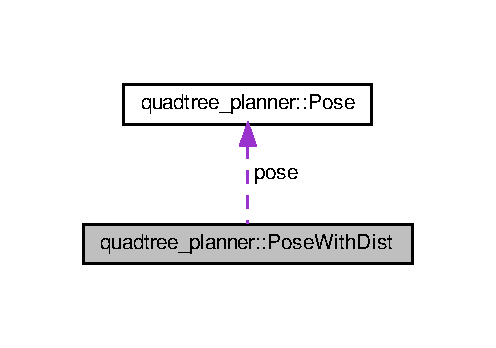
\includegraphics[width=238pt]{structquadtree__planner_1_1PoseWithDist__coll__graph}
\end{center}
\end{figure}
\subsection*{Public Member Functions}
\begin{DoxyCompactItemize}
\item 
\mbox{\Hypertarget{structquadtree__planner_1_1PoseWithDist_a4f444de5a17f206cb78af02b5f6f27d4}\label{structquadtree__planner_1_1PoseWithDist_a4f444de5a17f206cb78af02b5f6f27d4}} 
{\bfseries Pose\+With\+Dist} (double dist, const \hyperlink{structquadtree__planner_1_1Pose}{Pose} \&pose)
\item 
\mbox{\Hypertarget{structquadtree__planner_1_1PoseWithDist_a293ef50a7f2e827f426b0d0d154db673}\label{structquadtree__planner_1_1PoseWithDist_a293ef50a7f2e827f426b0d0d154db673}} 
bool {\bfseries operator$<$} (const \hyperlink{structquadtree__planner_1_1PoseWithDist}{Pose\+With\+Dist} \&other) const
\item 
\mbox{\Hypertarget{structquadtree__planner_1_1PoseWithDist_a1a3636f214ea3c2b8985d119a7b895e5}\label{structquadtree__planner_1_1PoseWithDist_a1a3636f214ea3c2b8985d119a7b895e5}} 
bool {\bfseries operator==} (const \hyperlink{structquadtree__planner_1_1PoseWithDist}{Pose\+With\+Dist} \&other) const
\end{DoxyCompactItemize}
\subsection*{Public Attributes}
\begin{DoxyCompactItemize}
\item 
\mbox{\Hypertarget{structquadtree__planner_1_1PoseWithDist_ab549c0b14696617a99075edad7d73610}\label{structquadtree__planner_1_1PoseWithDist_ab549c0b14696617a99075edad7d73610}} 
double {\bfseries dist}
\item 
\mbox{\Hypertarget{structquadtree__planner_1_1PoseWithDist_a191cde7579ae0af7f1fec2c731c34649}\label{structquadtree__planner_1_1PoseWithDist_a191cde7579ae0af7f1fec2c731c34649}} 
\hyperlink{structquadtree__planner_1_1Pose}{Pose} {\bfseries pose}
\end{DoxyCompactItemize}


\subsection{Detailed Description}
Container for storing object position and associated cost. 

The documentation for this struct was generated from the following files\+:\begin{DoxyCompactItemize}
\item 
/home/maximilian/\+Roboy\+Repo\+Devel\+Planning/src/quadtree\+\_\+planner/include/quadtree\+\_\+planner/utils.\+h\item 
/home/maximilian/\+Roboy\+Repo\+Devel\+Planning/src/quadtree\+\_\+planner/src/utils.\+cpp\end{DoxyCompactItemize}

\hypertarget{classQuadtree__Cell}{}\section{Quadtree\+\_\+\+Cell Class Reference}
\label{classQuadtree__Cell}\index{Quadtree\+\_\+\+Cell@{Quadtree\+\_\+\+Cell}}
\subsection*{Public Member Functions}
\begin{DoxyCompactItemize}
\item 
\mbox{\Hypertarget{classQuadtree__Cell_ad8e516e00e51b897ec5a26240c4b3373}\label{classQuadtree__Cell_ad8e516e00e51b897ec5a26240c4b3373}} 
{\bfseries Quadtree\+\_\+\+Cell} (\hyperlink{structPoint}{Point} \+\_\+topL, \hyperlink{structPoint}{Point} \+\_\+botR, unsigned int \+\_\+cost)
\item 
int \hyperlink{classQuadtree__Cell_af2b30e86c7180372b97177d43888210c}{build\+Quadtree} (\hyperlink{classquadtree__planner_1_1Costmap}{quadtree\+\_\+planner\+::\+Costmap} $\ast$costmap, long long $\ast$area\+\_\+)
\begin{DoxyCompactList}\small\item\em This method builds a quadtree datastructure based on a 2D costmap as input. It subdivides cells as long as they are not uniform yet (uniform means whole cell is free or whole cell is occupied). \end{DoxyCompactList}\item 
void \hyperlink{classQuadtree__Cell_a30ac8c78fb0693cd7c8e1631fd312426}{test\+Quadtree} (ros\+::\+Publisher marker\+\_\+publisher\+\_\+, double resolution, bool show\+Only\+Lowest\+Level, double origin\+\_\+x, double origin\+\_\+y)
\begin{DoxyCompactList}\small\item\em This method visualizes the quadtree cells in rviz. \end{DoxyCompactList}\item 
void \hyperlink{classQuadtree__Cell_ae121e7759a290d90f3b4ab12f4460b47}{create\+Search\+Cell\+Vector} (std\+::vector$<$ \hyperlink{classQuadtree__SearchCell}{Quadtree\+\_\+\+Search\+Cell} $>$ $\ast$quad\+Vector)
\begin{DoxyCompactList}\small\item\em Creates a std\+::vector with \hyperlink{classQuadtree__SearchCell}{Quadtree\+\_\+\+Search\+Cell} objects based on the \hyperlink{classQuadtree__Cell}{Quadtree\+\_\+\+Cell}. \end{DoxyCompactList}\item 
void \hyperlink{classQuadtree__Cell_aa3bad1fe80dbfc5b576e63635481e11d}{find\+Neighbors\+In\+Search\+Cell\+Vector} (std\+::vector$<$ \hyperlink{classQuadtree__SearchCell}{Quadtree\+\_\+\+Search\+Cell} $>$ \&quad\+Vector)
\begin{DoxyCompactList}\small\item\em Finds the neighbors of all Quadtree\+\_\+\+Search\+Cells contained in the input std\+::vector. \end{DoxyCompactList}\item 
\mbox{\Hypertarget{classQuadtree__Cell_a070aaa76b5c28fc1473d5943019e9fb8}\label{classQuadtree__Cell_a070aaa76b5c28fc1473d5943019e9fb8}} 
bool {\bfseries operator==} (const \hyperlink{classQuadtree__Cell}{Quadtree\+\_\+\+Cell} \&p) const
\item 
\mbox{\Hypertarget{classQuadtree__Cell_aedc198bc943d4d7214abd3b2477d95f5}\label{classQuadtree__Cell_aedc198bc943d4d7214abd3b2477d95f5}} 
void \hyperlink{classQuadtree__Cell_aedc198bc943d4d7214abd3b2477d95f5}{print\+Quadtree} ()
\begin{DoxyCompactList}\small\item\em Prints topL, botR and cost of the \hyperlink{classQuadtree__Cell}{Quadtree\+\_\+\+Cell} object. \end{DoxyCompactList}\end{DoxyCompactItemize}


\subsection{Member Function Documentation}
\mbox{\Hypertarget{classQuadtree__Cell_af2b30e86c7180372b97177d43888210c}\label{classQuadtree__Cell_af2b30e86c7180372b97177d43888210c}} 
\index{Quadtree\+\_\+\+Cell@{Quadtree\+\_\+\+Cell}!build\+Quadtree@{build\+Quadtree}}
\index{build\+Quadtree@{build\+Quadtree}!Quadtree\+\_\+\+Cell@{Quadtree\+\_\+\+Cell}}
\subsubsection{\texorpdfstring{build\+Quadtree()}{buildQuadtree()}}
{\footnotesize\ttfamily int Quadtree\+\_\+\+Cell\+::build\+Quadtree (\begin{DoxyParamCaption}\item[{\hyperlink{classquadtree__planner_1_1Costmap}{quadtree\+\_\+planner\+::\+Costmap} $\ast$}]{costmap,  }\item[{long long $\ast$}]{area\+\_\+ }\end{DoxyParamCaption})}



This method builds a quadtree datastructure based on a 2D costmap as input. It subdivides cells as long as they are not uniform yet (uniform means whole cell is free or whole cell is occupied). 


\begin{DoxyParams}{Parameters}
{\em costmap} & pointer to the costmap that is used to construct the quadtree \\
\hline
{\em area\+\_\+} & debug variable that stores the area of the whole quadtree \\
\hline
\end{DoxyParams}
\begin{DoxyReturn}{Returns}
0 if is creation succesful, -\/1 otherwise 
\end{DoxyReturn}
\mbox{\Hypertarget{classQuadtree__Cell_ae121e7759a290d90f3b4ab12f4460b47}\label{classQuadtree__Cell_ae121e7759a290d90f3b4ab12f4460b47}} 
\index{Quadtree\+\_\+\+Cell@{Quadtree\+\_\+\+Cell}!create\+Search\+Cell\+Vector@{create\+Search\+Cell\+Vector}}
\index{create\+Search\+Cell\+Vector@{create\+Search\+Cell\+Vector}!Quadtree\+\_\+\+Cell@{Quadtree\+\_\+\+Cell}}
\subsubsection{\texorpdfstring{create\+Search\+Cell\+Vector()}{createSearchCellVector()}}
{\footnotesize\ttfamily void Quadtree\+\_\+\+Cell\+::create\+Search\+Cell\+Vector (\begin{DoxyParamCaption}\item[{std\+::vector$<$ \hyperlink{classQuadtree__SearchCell}{Quadtree\+\_\+\+Search\+Cell} $>$ $\ast$}]{quad\+Vector }\end{DoxyParamCaption})}



Creates a std\+::vector with \hyperlink{classQuadtree__SearchCell}{Quadtree\+\_\+\+Search\+Cell} objects based on the \hyperlink{classQuadtree__Cell}{Quadtree\+\_\+\+Cell}. 


\begin{DoxyParams}{Parameters}
{\em quad\+Vector} & std\+::vector to store the \hyperlink{classQuadtree__SearchCell}{Quadtree\+\_\+\+Search\+Cell} objects \\
\hline
\end{DoxyParams}
\mbox{\Hypertarget{classQuadtree__Cell_aa3bad1fe80dbfc5b576e63635481e11d}\label{classQuadtree__Cell_aa3bad1fe80dbfc5b576e63635481e11d}} 
\index{Quadtree\+\_\+\+Cell@{Quadtree\+\_\+\+Cell}!find\+Neighbors\+In\+Search\+Cell\+Vector@{find\+Neighbors\+In\+Search\+Cell\+Vector}}
\index{find\+Neighbors\+In\+Search\+Cell\+Vector@{find\+Neighbors\+In\+Search\+Cell\+Vector}!Quadtree\+\_\+\+Cell@{Quadtree\+\_\+\+Cell}}
\subsubsection{\texorpdfstring{find\+Neighbors\+In\+Search\+Cell\+Vector()}{findNeighborsInSearchCellVector()}}
{\footnotesize\ttfamily void Quadtree\+\_\+\+Cell\+::find\+Neighbors\+In\+Search\+Cell\+Vector (\begin{DoxyParamCaption}\item[{std\+::vector$<$ \hyperlink{classQuadtree__SearchCell}{Quadtree\+\_\+\+Search\+Cell} $>$ \&}]{quad\+Vector }\end{DoxyParamCaption})}



Finds the neighbors of all Quadtree\+\_\+\+Search\+Cells contained in the input std\+::vector. 


\begin{DoxyParams}{Parameters}
{\em quad\+Vector} & neighbors of Quadtree\+\_\+\+Search\+Cells in this vector are found and set by this method \\
\hline
\end{DoxyParams}
\mbox{\Hypertarget{classQuadtree__Cell_a30ac8c78fb0693cd7c8e1631fd312426}\label{classQuadtree__Cell_a30ac8c78fb0693cd7c8e1631fd312426}} 
\index{Quadtree\+\_\+\+Cell@{Quadtree\+\_\+\+Cell}!test\+Quadtree@{test\+Quadtree}}
\index{test\+Quadtree@{test\+Quadtree}!Quadtree\+\_\+\+Cell@{Quadtree\+\_\+\+Cell}}
\subsubsection{\texorpdfstring{test\+Quadtree()}{testQuadtree()}}
{\footnotesize\ttfamily void Quadtree\+\_\+\+Cell\+::test\+Quadtree (\begin{DoxyParamCaption}\item[{ros\+::\+Publisher}]{marker\+\_\+publisher\+\_\+,  }\item[{double}]{resolution,  }\item[{bool}]{show\+Only\+Lowest\+Level,  }\item[{double}]{origin\+\_\+x,  }\item[{double}]{origin\+\_\+y }\end{DoxyParamCaption})}



This method visualizes the quadtree cells in rviz. 


\begin{DoxyParams}{Parameters}
{\em marker\+\_\+publisher\+\_\+} & ros\+::publisher to publish the cells as markers to rviz \\
\hline
{\em resolution} & resolution of the costmap in meters per cell \\
\hline
{\em show\+Only\+Lowest\+Level} & if true, show only the lowest level of the quadtree \\
\hline
{\em origin\+\_\+x} & origin in x direction of costmap in meters \\
\hline
{\em origin\+\_\+y\+\_\+origin} & in y direction of costmap in meters \\
\hline
\end{DoxyParams}


The documentation for this class was generated from the following files\+:\begin{DoxyCompactItemize}
\item 
/home/maximilian/\+Roboy\+Repo\+Devel\+Planning/src/quadtree\+\_\+planner/include/quadtree\+\_\+planner/quadtree\+\_\+datastructure.\+h\item 
/home/maximilian/\+Roboy\+Repo\+Devel\+Planning/src/quadtree\+\_\+planner/src/quadtree\+\_\+datastructure.\+cpp\end{DoxyCompactItemize}

\hypertarget{classQuadtree__SearchCell}{}\section{Quadtree\+\_\+\+Search\+Cell Class Reference}
\label{classQuadtree__SearchCell}\index{Quadtree\+\_\+\+Search\+Cell@{Quadtree\+\_\+\+Search\+Cell}}


{\ttfamily \#include $<$quadtree\+\_\+datastructure.\+h$>$}



Collaboration diagram for Quadtree\+\_\+\+Search\+Cell\+:\nopagebreak
\begin{figure}[H]
\begin{center}
\leavevmode
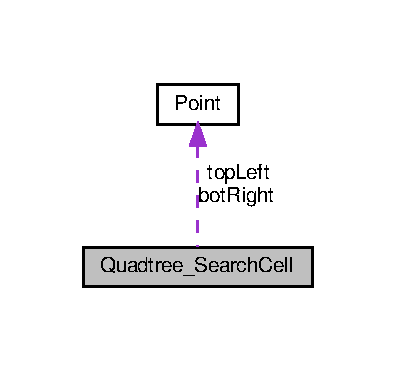
\includegraphics[width=190pt]{classQuadtree__SearchCell__coll__graph}
\end{center}
\end{figure}
\subsection*{Public Member Functions}
\begin{DoxyCompactItemize}
\item 
\mbox{\Hypertarget{classQuadtree__SearchCell_aae69ecac827985bc95c5d93736a874bf}\label{classQuadtree__SearchCell_aae69ecac827985bc95c5d93736a874bf}} 
{\bfseries Quadtree\+\_\+\+Search\+Cell} (\hyperlink{structPoint}{Point} \+\_\+topL, \hyperlink{structPoint}{Point} \+\_\+botR, unsigned int \+\_\+cost, std\+::vector$<$ \hyperlink{classQuadtree__SearchCell}{Quadtree\+\_\+\+Search\+Cell} $\ast$$>$ \+\_\+neighbors)
\item 
\mbox{\Hypertarget{classQuadtree__SearchCell_ad19965518209ded935963af6f82439b0}\label{classQuadtree__SearchCell_ad19965518209ded935963af6f82439b0}} 
bool {\bfseries operator==} (const \hyperlink{classQuadtree__SearchCell}{Quadtree\+\_\+\+Search\+Cell} \&other) const
\item 
\hyperlink{structPoint}{Point} \hyperlink{classQuadtree__SearchCell_a757563b6c0b2c46ab3470225fc3d9026}{get\+Top\+Left} ()
\begin{DoxyCompactList}\small\item\em Returns the top left point of the quadtree search cell. \end{DoxyCompactList}\item 
\hyperlink{structPoint}{Point} \hyperlink{classQuadtree__SearchCell_aa05145ed327cd4043027ea7d0dc05006}{get\+Bot\+Right} ()
\begin{DoxyCompactList}\small\item\em Returns the bottom right point of the quadtree search cell. \end{DoxyCompactList}\item 
unsigned int \hyperlink{classQuadtree__SearchCell_af5398942f7a48fc146ec99f798aedc71}{get\+Cost} ()
\begin{DoxyCompactList}\small\item\em returns the cost of the quadtree search cell \end{DoxyCompactList}\item 
std\+::vector$<$ \hyperlink{classQuadtree__SearchCell}{Quadtree\+\_\+\+Search\+Cell} $\ast$ $>$ \hyperlink{classQuadtree__SearchCell_a8af6b597f8a32c7c19f858f34d16efa2}{get\+Neighbors} ()
\begin{DoxyCompactList}\small\item\em Returns a std\+::vector of pointers to the neighbors of this quadtree search cell. \end{DoxyCompactList}\item 
void \hyperlink{classQuadtree__SearchCell_a36c9e92db030bb40f563d0c3b0453c8b}{set\+Neighbors} (std\+::vector$<$ \hyperlink{classQuadtree__SearchCell}{Quadtree\+\_\+\+Search\+Cell} $\ast$$>$ \+\_\+neighbors)
\begin{DoxyCompactList}\small\item\em Sets a std\+::vector of pointers to the neighbors of this quadtree search cell. \end{DoxyCompactList}\end{DoxyCompactItemize}
\subsection*{Public Attributes}
\begin{DoxyCompactItemize}
\item 
\mbox{\Hypertarget{classQuadtree__SearchCell_a5364a5cc75d4eaaafdd2e96a679b8073}\label{classQuadtree__SearchCell_a5364a5cc75d4eaaafdd2e96a679b8073}} 
\hyperlink{structPoint}{Point} {\bfseries top\+Left}
\item 
\mbox{\Hypertarget{classQuadtree__SearchCell_a39b17158a3eca5ba37dc5f850a1283d5}\label{classQuadtree__SearchCell_a39b17158a3eca5ba37dc5f850a1283d5}} 
\hyperlink{structPoint}{Point} {\bfseries bot\+Right}
\item 
\mbox{\Hypertarget{classQuadtree__SearchCell_a6377f42344a7108ec70768b2f8ebe83e}\label{classQuadtree__SearchCell_a6377f42344a7108ec70768b2f8ebe83e}} 
unsigned int {\bfseries cost}
\item 
\mbox{\Hypertarget{classQuadtree__SearchCell_ae633f7a72335bb2c13420667bb34ec1c}\label{classQuadtree__SearchCell_ae633f7a72335bb2c13420667bb34ec1c}} 
std\+::vector$<$ \hyperlink{classQuadtree__SearchCell}{Quadtree\+\_\+\+Search\+Cell} $\ast$ $>$ {\bfseries neighbors}
\end{DoxyCompactItemize}


\subsection{Detailed Description}
used as nodes in the A$\ast$ search algorithm 

\subsection{Member Function Documentation}
\mbox{\Hypertarget{classQuadtree__SearchCell_aa05145ed327cd4043027ea7d0dc05006}\label{classQuadtree__SearchCell_aa05145ed327cd4043027ea7d0dc05006}} 
\index{Quadtree\+\_\+\+Search\+Cell@{Quadtree\+\_\+\+Search\+Cell}!get\+Bot\+Right@{get\+Bot\+Right}}
\index{get\+Bot\+Right@{get\+Bot\+Right}!Quadtree\+\_\+\+Search\+Cell@{Quadtree\+\_\+\+Search\+Cell}}
\subsubsection{\texorpdfstring{get\+Bot\+Right()}{getBotRight()}}
{\footnotesize\ttfamily \hyperlink{structPoint}{Point} Quadtree\+\_\+\+Search\+Cell\+::get\+Bot\+Right (\begin{DoxyParamCaption}{ }\end{DoxyParamCaption})}



Returns the bottom right point of the quadtree search cell. 

\begin{DoxyReturn}{Returns}
bottom right point of the quadtree search cell 
\end{DoxyReturn}
\mbox{\Hypertarget{classQuadtree__SearchCell_af5398942f7a48fc146ec99f798aedc71}\label{classQuadtree__SearchCell_af5398942f7a48fc146ec99f798aedc71}} 
\index{Quadtree\+\_\+\+Search\+Cell@{Quadtree\+\_\+\+Search\+Cell}!get\+Cost@{get\+Cost}}
\index{get\+Cost@{get\+Cost}!Quadtree\+\_\+\+Search\+Cell@{Quadtree\+\_\+\+Search\+Cell}}
\subsubsection{\texorpdfstring{get\+Cost()}{getCost()}}
{\footnotesize\ttfamily unsigned int Quadtree\+\_\+\+Search\+Cell\+::get\+Cost (\begin{DoxyParamCaption}{ }\end{DoxyParamCaption})}



returns the cost of the quadtree search cell 

\begin{DoxyReturn}{Returns}
cost of the quadtree search cell 
\end{DoxyReturn}
\mbox{\Hypertarget{classQuadtree__SearchCell_a8af6b597f8a32c7c19f858f34d16efa2}\label{classQuadtree__SearchCell_a8af6b597f8a32c7c19f858f34d16efa2}} 
\index{Quadtree\+\_\+\+Search\+Cell@{Quadtree\+\_\+\+Search\+Cell}!get\+Neighbors@{get\+Neighbors}}
\index{get\+Neighbors@{get\+Neighbors}!Quadtree\+\_\+\+Search\+Cell@{Quadtree\+\_\+\+Search\+Cell}}
\subsubsection{\texorpdfstring{get\+Neighbors()}{getNeighbors()}}
{\footnotesize\ttfamily std\+::vector$<$ \hyperlink{classQuadtree__SearchCell}{Quadtree\+\_\+\+Search\+Cell} $\ast$ $>$ Quadtree\+\_\+\+Search\+Cell\+::get\+Neighbors (\begin{DoxyParamCaption}{ }\end{DoxyParamCaption})}



Returns a std\+::vector of pointers to the neighbors of this quadtree search cell. 

\begin{DoxyReturn}{Returns}
a std\+::vector of pointers to the neighbors of this quadtree search cell 
\end{DoxyReturn}
\mbox{\Hypertarget{classQuadtree__SearchCell_a757563b6c0b2c46ab3470225fc3d9026}\label{classQuadtree__SearchCell_a757563b6c0b2c46ab3470225fc3d9026}} 
\index{Quadtree\+\_\+\+Search\+Cell@{Quadtree\+\_\+\+Search\+Cell}!get\+Top\+Left@{get\+Top\+Left}}
\index{get\+Top\+Left@{get\+Top\+Left}!Quadtree\+\_\+\+Search\+Cell@{Quadtree\+\_\+\+Search\+Cell}}
\subsubsection{\texorpdfstring{get\+Top\+Left()}{getTopLeft()}}
{\footnotesize\ttfamily \hyperlink{structPoint}{Point} Quadtree\+\_\+\+Search\+Cell\+::get\+Top\+Left (\begin{DoxyParamCaption}{ }\end{DoxyParamCaption})}



Returns the top left point of the quadtree search cell. 

\begin{DoxyReturn}{Returns}
top left point of the quadtree search cell 
\end{DoxyReturn}
\mbox{\Hypertarget{classQuadtree__SearchCell_a36c9e92db030bb40f563d0c3b0453c8b}\label{classQuadtree__SearchCell_a36c9e92db030bb40f563d0c3b0453c8b}} 
\index{Quadtree\+\_\+\+Search\+Cell@{Quadtree\+\_\+\+Search\+Cell}!set\+Neighbors@{set\+Neighbors}}
\index{set\+Neighbors@{set\+Neighbors}!Quadtree\+\_\+\+Search\+Cell@{Quadtree\+\_\+\+Search\+Cell}}
\subsubsection{\texorpdfstring{set\+Neighbors()}{setNeighbors()}}
{\footnotesize\ttfamily void Quadtree\+\_\+\+Search\+Cell\+::set\+Neighbors (\begin{DoxyParamCaption}\item[{std\+::vector$<$ \hyperlink{classQuadtree__SearchCell}{Quadtree\+\_\+\+Search\+Cell} $\ast$$>$}]{\+\_\+neighbors }\end{DoxyParamCaption})}



Sets a std\+::vector of pointers to the neighbors of this quadtree search cell. 


\begin{DoxyParams}{Parameters}
{\em \+\_\+neighbors} & std\+::vector of pointers to the neighbors of this quadtree search cell \\
\hline
\end{DoxyParams}


The documentation for this class was generated from the following files\+:\begin{DoxyCompactItemize}
\item 
/home/maximilian/\+Roboy\+Repo\+Devel\+Planning/src/quadtree\+\_\+planner/include/quadtree\+\_\+planner/quadtree\+\_\+datastructure.\+h\item 
/home/maximilian/\+Roboy\+Repo\+Devel\+Planning/src/quadtree\+\_\+planner/src/quadtree\+\_\+datastructure.\+cpp\end{DoxyCompactItemize}

\hypertarget{structquadtree__planner_1_1QuadtreeCellWithDist}{}\section{quadtree\+\_\+planner\+:\+:Quadtree\+Cell\+With\+Dist Struct Reference}
\label{structquadtree__planner_1_1QuadtreeCellWithDist}\index{quadtree\+\_\+planner\+::\+Quadtree\+Cell\+With\+Dist@{quadtree\+\_\+planner\+::\+Quadtree\+Cell\+With\+Dist}}


{\ttfamily \#include $<$utils.\+h$>$}



Collaboration diagram for quadtree\+\_\+planner\+:\+:Quadtree\+Cell\+With\+Dist\+:\nopagebreak
\begin{figure}[H]
\begin{center}
\leavevmode
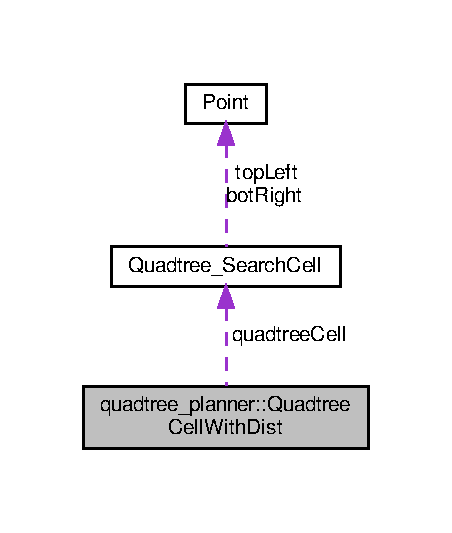
\includegraphics[width=217pt]{structquadtree__planner_1_1QuadtreeCellWithDist__coll__graph}
\end{center}
\end{figure}
\subsection*{Public Member Functions}
\begin{DoxyCompactItemize}
\item 
\mbox{\Hypertarget{structquadtree__planner_1_1QuadtreeCellWithDist_a9cb3e694743f7fbd8aa3cce7bc1922f7}\label{structquadtree__planner_1_1QuadtreeCellWithDist_a9cb3e694743f7fbd8aa3cce7bc1922f7}} 
{\bfseries Quadtree\+Cell\+With\+Dist} (double dist, \hyperlink{classQuadtree__SearchCell}{Quadtree\+\_\+\+Search\+Cell} \&quad)
\item 
\mbox{\Hypertarget{structquadtree__planner_1_1QuadtreeCellWithDist_a16c9b514ab8a8413b406a2dd36d2fa6c}\label{structquadtree__planner_1_1QuadtreeCellWithDist_a16c9b514ab8a8413b406a2dd36d2fa6c}} 
bool {\bfseries operator$<$} (const \hyperlink{structquadtree__planner_1_1QuadtreeCellWithDist}{Quadtree\+Cell\+With\+Dist} \&other) const
\item 
\mbox{\Hypertarget{structquadtree__planner_1_1QuadtreeCellWithDist_a554863dd5ddc8549717eb362f7de96f2}\label{structquadtree__planner_1_1QuadtreeCellWithDist_a554863dd5ddc8549717eb362f7de96f2}} 
bool {\bfseries operator==} (const \hyperlink{structquadtree__planner_1_1QuadtreeCellWithDist}{Quadtree\+Cell\+With\+Dist} \&other) const
\end{DoxyCompactItemize}
\subsection*{Public Attributes}
\begin{DoxyCompactItemize}
\item 
\mbox{\Hypertarget{structquadtree__planner_1_1QuadtreeCellWithDist_a640a4291ae6ee693a18377a8fe2e2081}\label{structquadtree__planner_1_1QuadtreeCellWithDist_a640a4291ae6ee693a18377a8fe2e2081}} 
double {\bfseries dist}
\item 
\mbox{\Hypertarget{structquadtree__planner_1_1QuadtreeCellWithDist_a3691048d0b7914d5a69932ce785b3a74}\label{structquadtree__planner_1_1QuadtreeCellWithDist_a3691048d0b7914d5a69932ce785b3a74}} 
\hyperlink{classQuadtree__SearchCell}{Quadtree\+\_\+\+Search\+Cell} {\bfseries quadtree\+Cell}
\end{DoxyCompactItemize}


\subsection{Detailed Description}
Container for storing quadtree cells and associated cost 

The documentation for this struct was generated from the following files\+:\begin{DoxyCompactItemize}
\item 
/home/maximilian/\+Roboy\+Repo\+Devel\+Planning/src/quadtree\+\_\+planner/include/quadtree\+\_\+planner/utils.\+h\item 
/home/maximilian/\+Roboy\+Repo\+Devel\+Planning/src/quadtree\+\_\+planner/src/utils.\+cpp\end{DoxyCompactItemize}

\hypertarget{classquadtree__planner_1_1QuadTreePlanner}{}\section{quadtree\+\_\+planner\+:\+:Quad\+Tree\+Planner Class Reference}
\label{classquadtree__planner_1_1QuadTreePlanner}\index{quadtree\+\_\+planner\+::\+Quad\+Tree\+Planner@{quadtree\+\_\+planner\+::\+Quad\+Tree\+Planner}}


Inheritance diagram for quadtree\+\_\+planner\+:\+:Quad\+Tree\+Planner\+:\nopagebreak
\begin{figure}[H]
\begin{center}
\leavevmode
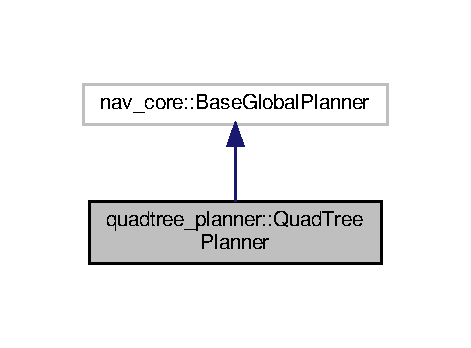
\includegraphics[width=226pt]{classquadtree__planner_1_1QuadTreePlanner__inherit__graph}
\end{center}
\end{figure}


Collaboration diagram for quadtree\+\_\+planner\+:\+:Quad\+Tree\+Planner\+:\nopagebreak
\begin{figure}[H]
\begin{center}
\leavevmode
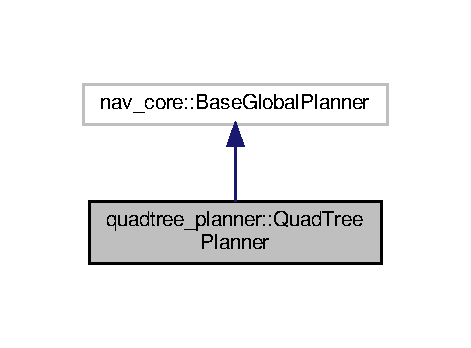
\includegraphics[width=226pt]{classquadtree__planner_1_1QuadTreePlanner__coll__graph}
\end{center}
\end{figure}
\subsection*{Public Member Functions}
\begin{DoxyCompactItemize}
\item 
void \hyperlink{classquadtree__planner_1_1QuadTreePlanner_a95b6b962b0bb8b7cb3a823d853ad447f}{initialize} (std\+::string name, costmap\+\_\+2d\+::\+Costmap2\+D\+R\+OS $\ast$costmap\+\_\+ros) override
\item 
bool \hyperlink{classquadtree__planner_1_1QuadTreePlanner_a65ced31e9ea72cbee760f593f47115cd}{make\+Plan} (const geometry\+\_\+msgs\+::\+Pose\+Stamped \&start, const geometry\+\_\+msgs\+::\+Pose\+Stamped \&goal, std\+::vector$<$ geometry\+\_\+msgs\+::\+Pose\+Stamped $>$ \&plan) override
\item 
void \hyperlink{classquadtree__planner_1_1QuadTreePlanner_a6bc83db035560028672f572a985d05b7}{initialize} (std\+::string name, \hyperlink{classquadtree__planner_1_1Costmap}{Costmap} $\ast$costmap)
\item 
bool \hyperlink{classquadtree__planner_1_1QuadTreePlanner_a6f194e11417938fd90bcc74bcb578dca}{make\+Plan} (const \hyperlink{structquadtree__planner_1_1Pose}{Pose} \&start, const \hyperlink{structquadtree__planner_1_1Pose}{Pose} \&goal, std\+::vector$<$ \hyperlink{structquadtree__planner_1_1Pose}{Pose} $>$ \&path)
\end{DoxyCompactItemize}


\subsection{Member Function Documentation}
\mbox{\Hypertarget{classquadtree__planner_1_1QuadTreePlanner_a95b6b962b0bb8b7cb3a823d853ad447f}\label{classquadtree__planner_1_1QuadTreePlanner_a95b6b962b0bb8b7cb3a823d853ad447f}} 
\index{quadtree\+\_\+planner\+::\+Quad\+Tree\+Planner@{quadtree\+\_\+planner\+::\+Quad\+Tree\+Planner}!initialize@{initialize}}
\index{initialize@{initialize}!quadtree\+\_\+planner\+::\+Quad\+Tree\+Planner@{quadtree\+\_\+planner\+::\+Quad\+Tree\+Planner}}
\subsubsection{\texorpdfstring{initialize()}{initialize()}\hspace{0.1cm}{\footnotesize\ttfamily [1/2]}}
{\footnotesize\ttfamily void quadtree\+\_\+planner\+::\+Quad\+Tree\+Planner\+::initialize (\begin{DoxyParamCaption}\item[{std\+::string}]{name,  }\item[{costmap\+\_\+2d\+::\+Costmap2\+D\+R\+OS $\ast$}]{costmap\+\_\+ros }\end{DoxyParamCaption})\hspace{0.3cm}{\ttfamily [override]}}

Initialization function for the \hyperlink{classquadtree__planner_1_1QuadTreePlanner}{Quad\+Tree\+Planner} object 
\begin{DoxyParams}{Parameters}
{\em name} & The name of this planner \\
\hline
{\em costmap\+\_\+ros} & A pointer to the R\+OS wrapper of the costmap to use \\
\hline
\end{DoxyParams}
\mbox{\Hypertarget{classquadtree__planner_1_1QuadTreePlanner_a6bc83db035560028672f572a985d05b7}\label{classquadtree__planner_1_1QuadTreePlanner_a6bc83db035560028672f572a985d05b7}} 
\index{quadtree\+\_\+planner\+::\+Quad\+Tree\+Planner@{quadtree\+\_\+planner\+::\+Quad\+Tree\+Planner}!initialize@{initialize}}
\index{initialize@{initialize}!quadtree\+\_\+planner\+::\+Quad\+Tree\+Planner@{quadtree\+\_\+planner\+::\+Quad\+Tree\+Planner}}
\subsubsection{\texorpdfstring{initialize()}{initialize()}\hspace{0.1cm}{\footnotesize\ttfamily [2/2]}}
{\footnotesize\ttfamily void quadtree\+\_\+planner\+::\+Quad\+Tree\+Planner\+::initialize (\begin{DoxyParamCaption}\item[{std\+::string}]{name,  }\item[{\hyperlink{classquadtree__planner_1_1Costmap}{quadtree\+\_\+planner\+::\+Costmap} $\ast$}]{costmap }\end{DoxyParamCaption})}

Initialization function for the \hyperlink{classquadtree__planner_1_1QuadTreePlanner}{Quad\+Tree\+Planner} object 
\begin{DoxyParams}{Parameters}
{\em name} & The name of this planner \\
\hline
{\em costmap} & a pointer to the costmap to use \\
\hline
\end{DoxyParams}
\mbox{\Hypertarget{classquadtree__planner_1_1QuadTreePlanner_a65ced31e9ea72cbee760f593f47115cd}\label{classquadtree__planner_1_1QuadTreePlanner_a65ced31e9ea72cbee760f593f47115cd}} 
\index{quadtree\+\_\+planner\+::\+Quad\+Tree\+Planner@{quadtree\+\_\+planner\+::\+Quad\+Tree\+Planner}!make\+Plan@{make\+Plan}}
\index{make\+Plan@{make\+Plan}!quadtree\+\_\+planner\+::\+Quad\+Tree\+Planner@{quadtree\+\_\+planner\+::\+Quad\+Tree\+Planner}}
\subsubsection{\texorpdfstring{make\+Plan()}{makePlan()}\hspace{0.1cm}{\footnotesize\ttfamily [1/2]}}
{\footnotesize\ttfamily bool quadtree\+\_\+planner\+::\+Quad\+Tree\+Planner\+::make\+Plan (\begin{DoxyParamCaption}\item[{const geometry\+\_\+msgs\+::\+Pose\+Stamped \&}]{start,  }\item[{const geometry\+\_\+msgs\+::\+Pose\+Stamped \&}]{goal,  }\item[{std\+::vector$<$ geometry\+\_\+msgs\+::\+Pose\+Stamped $>$ \&}]{plan }\end{DoxyParamCaption})\hspace{0.3cm}{\ttfamily [override]}}

Given a goal pose in the world, compute a plan 
\begin{DoxyParams}{Parameters}
{\em start} & The start pose \\
\hline
{\em goal} & The goal pose \\
\hline
{\em plan} & The plan... filled by the planner \\
\hline
\end{DoxyParams}
\begin{DoxyReturn}{Returns}
True if a valid plan was found, false otherwise 
\end{DoxyReturn}
\mbox{\Hypertarget{classquadtree__planner_1_1QuadTreePlanner_a6f194e11417938fd90bcc74bcb578dca}\label{classquadtree__planner_1_1QuadTreePlanner_a6f194e11417938fd90bcc74bcb578dca}} 
\index{quadtree\+\_\+planner\+::\+Quad\+Tree\+Planner@{quadtree\+\_\+planner\+::\+Quad\+Tree\+Planner}!make\+Plan@{make\+Plan}}
\index{make\+Plan@{make\+Plan}!quadtree\+\_\+planner\+::\+Quad\+Tree\+Planner@{quadtree\+\_\+planner\+::\+Quad\+Tree\+Planner}}
\subsubsection{\texorpdfstring{make\+Plan()}{makePlan()}\hspace{0.1cm}{\footnotesize\ttfamily [2/2]}}
{\footnotesize\ttfamily bool quadtree\+\_\+planner\+::\+Quad\+Tree\+Planner\+::make\+Plan (\begin{DoxyParamCaption}\item[{const \hyperlink{structquadtree__planner_1_1Pose}{Pose} \&}]{start,  }\item[{const \hyperlink{structquadtree__planner_1_1Pose}{Pose} \&}]{goal,  }\item[{std\+::vector$<$ \hyperlink{structquadtree__planner_1_1Pose}{Pose} $>$ \&}]{path }\end{DoxyParamCaption})}

Given a goal pose in the world, compute a plan 
\begin{DoxyParams}{Parameters}
{\em start} & The start pose \\
\hline
{\em goal} & The goal pose \\
\hline
{\em plan} & The plan... filled by the planner \\
\hline
\end{DoxyParams}
\begin{DoxyReturn}{Returns}
True if a valid plan was found, false otherwise 
\end{DoxyReturn}


The documentation for this class was generated from the following files\+:\begin{DoxyCompactItemize}
\item 
/home/maximilian/\+Roboy\+Repo\+Devel\+Planning/src/quadtree\+\_\+planner/include/quadtree\+\_\+planner/quadtree\+\_\+planner.\+h\item 
/home/maximilian/\+Roboy\+Repo\+Devel\+Planning/src/quadtree\+\_\+planner/src/quadtree\+\_\+planner.\+cpp\end{DoxyCompactItemize}

%--- End generated contents ---

% Index
\backmatter
\newpage
\phantomsection
\clearemptydoublepage
\addcontentsline{toc}{chapter}{Index}
\printindex

\end{document}
